\documentclass[9pt,a4paper,twocolumn,twoside]{tau-class/tau}
\usepackage[spanish,es-nodecimaldot,es-noindentfirst]{babel}
\usepackage{booktabs}
\usepackage{longtable}
\usepackage{hyperref}
\usepackage{graphicx}

\graphicspath{{figures/netplus-loja/}}

\doctype{Reporte competitivo}
\title{Analisis competitivo de NETPLUS en Loja (Ecuador)}
\author[a,1]{Equipo de Analitica Oderbiz}
\affil[a]{Unidad de Inteligencia Comercial}
\dates{Compilado el \today}
\docinfo{Documento elaborado con evidencia publica en sitios oficiales y redes sociales. Todo dato observado esta marcado como \texttt{observado}. Toda conclusion analitica esta marcada como \texttt{inferencia}.}
\footinfo{Reporte Oderbiz}
\theday{\today}
\organization{Oderbiz}
\leadauthor{Equipo Oderbiz}

\begin{abstract}
Se analizo la posicion de NETPLUS frente a Velocity, Celerity, CNT, Vilcanet, Netlife, Xtrim y Snel en la ciudad de Loja, con foco en visibilidad digital, propuesta comercial, precios publicos y actividad en redes (\texttt{observado}). Los competidores nacionales (CNT, Netlife, Xtrim) muestran mayor escala de marca y estructura comercial visible (\texttt{observado}). Los operadores regionales (Velocity, Vilcanet, Snel, y perfiles locales asociados a Celerity) compiten por cercania, promociones y respuesta operativa (\texttt{observado}). Para NETPLUS, la principal oportunidad es convertir su identidad local en una ventaja comercial clara: propuesta de valor simple, pruebas sociales de clientes y captacion con seguimiento por WhatsApp (\texttt{inferencia}).
\end{abstract}

\keywords{internet fijo, fibra optica, Loja, Ecuador, competencia, redes sociales}

\begin{document}
\maketitle
\thispagestyle{firststyle}

\section{Contexto}
\textbf{Negocio analizado:} NETPLUS (Loja, Ecuador) (\texttt{observado}, indicado por cliente).\\
\textbf{Competidores solicitados:} Velocity, Celerity, CNT, Vilcanet, Netlife, Xtrim, Snel (\texttt{observado}).

\section{Matriz comparativa resumida}
\begin{table*}[t]
  \centering
  \small
  \begin{tabular}{@{}p{2.3cm}p{2.9cm}p{2.8cm}p{2.8cm}p{2.8cm}@{}}
    \toprule
    \textbf{Marca} & \textbf{Web oficial} & \textbf{Precio/planes visibles} & \textbf{Facebook} & \textbf{Lectura competitiva} \\
    \midrule
    NETPLUS & \url{https://www.nettplus.net/} (\texttt{obs}) & Plan visible en portada (700 Mbps y promo) (\texttt{obs}) & URL probada \url{https://www.facebook.com/nettplus.ec/} sin contenido publico (\texttt{obs}) & Marca local con potencial de cercania; necesita mayor estructura de captacion digital (\texttt{inf}) \\
    Velocity & \url{https://velocity.ec/} (\texttt{obs}) & Planes y narrativa comercial visible (\texttt{obs}) & \url{https://www.facebook.com/velocity.ec/} activo, 8k+ seguidores (\texttt{obs}) & Buena presencia regional y comunicacion frecuente (\texttt{inf}) \\
    Celerity & \url{https://www.celerity.ec/} (\texttt{obs}) & Planes/promociones visibles (\texttt{obs}) & \url{https://www.facebook.com/celerityec/} (perfil detectado) (\texttt{obs}) & Compite por promo y precio en mensajes (\texttt{inf}) \\
    CNT & \url{https://www.cnt.com.ec/productos/planes-internet} (\texttt{obs}) & Portafolio amplio y precios de entrada (\texttt{obs}) & \url{https://www.facebook.com/CNTEcuador/} verificada, 631k seguidores (\texttt{obs}) & Fuerte por marca pais y escala (\texttt{inf}) \\
    Vilcanet & \url{https://vilcanet.com/} (\texttt{obs}) & Planes 300/500/700 Mbps visibles (\texttt{obs}) & \url{https://www.facebook.com/vilcanet/} activo, 2.4k+ seguidores (\texttt{obs}) & Competidor local/regional directo (\texttt{inf}) \\
    Netlife & \url{https://netlife.ec/planes-hogar/} (\texttt{obs}) & Planes y descuentos por facturas visibles (\texttt{obs}) & URL evaluada \url{https://www.facebook.com/netlifeec/} no corresponde al perfil corporativo principal (\texttt{obs}) & Marca nacional fuerte en percepcion tecnologica (\texttt{inf}) \\
    Xtrim & \url{https://www.xtrim.com.ec/internet} (\texttt{obs}) & Oferta comercial agresiva y bundles (\texttt{obs}) & \url{https://www.facebook.com/xtrimecuador/} activo, 156k seguidores (\texttt{obs}) & Alta presion promocional y volumen (\texttt{inf}) \\
    Snel & \url{https://etelnetsol.com/planes-2025/} (\texttt{obs}) & Planes y requisitos visibles (\texttt{obs}) & No se confirmo perfil oficial en esta corrida (\texttt{obs}) & Juega por cercania y servicio local (\texttt{inf}) \\
    \bottomrule
  \end{tabular}
  \caption{Comparativo digital resumido (corte: 2026-05-05).}
\end{table*}

\section{Fortalezas y debilidades de NETPLUS}
\subsection{Fortalezas (\texttt{inferencia})}
\begin{itemize}
  \item Ventaja local: mayor potencial de confianza de barrio y trato cercano.
  \item Flexibilidad comercial para ajustar planes/promociones rapidamente.
  \item Espacio para diferenciarse por soporte tecnico y tiempos de atencion.
\end{itemize}

\subsection{Debilidades (\texttt{inferencia})}
\begin{itemize}
  \item Menor escala de marca frente a CNT, Netlife y Xtrim.
  \item Menor estandarizacion digital de canales sociales visibles.
  \item Riesgo de comparacion por precio sin defender valor de servicio local.
\end{itemize}

\section{Como potenciar ventas de NETPLUS}
\subsection*{P1 (alto impacto, bajo esfuerzo)}
\begin{itemize}
  \item Definir 3 planes ancla con mensaje simple: Economico / Hogar / Alto consumo.
  \item Campana de captacion local con CTA directo a WhatsApp y SLA de respuesta.
  \item Publicar testimonios reales por sector de Loja (con nombre y parroquia/zona).
\end{itemize}

\subsection*{P2 (alto impacto, esfuerzo medio)}
\begin{itemize}
  \item Comparativo comercial ``NETPLUS vs mercado'' centrado en servicio y cercania.
  \item Ofertas de cambio de operador: instalacion prioritaria + bono de bienvenida.
  \item Script comercial unificado para cierre: cobertura, velocidad real, soporte.
\end{itemize}

\subsection*{P3 (experimental)}
\begin{itemize}
  \item Programa de referidos con incentivo por alta efectiva.
  \item Campanas por microsegmento: teletrabajo, gamers, familias, pymes barriales.
\end{itemize}

\section{Evidencia visual}
\begin{figure}[h]
  \centering
  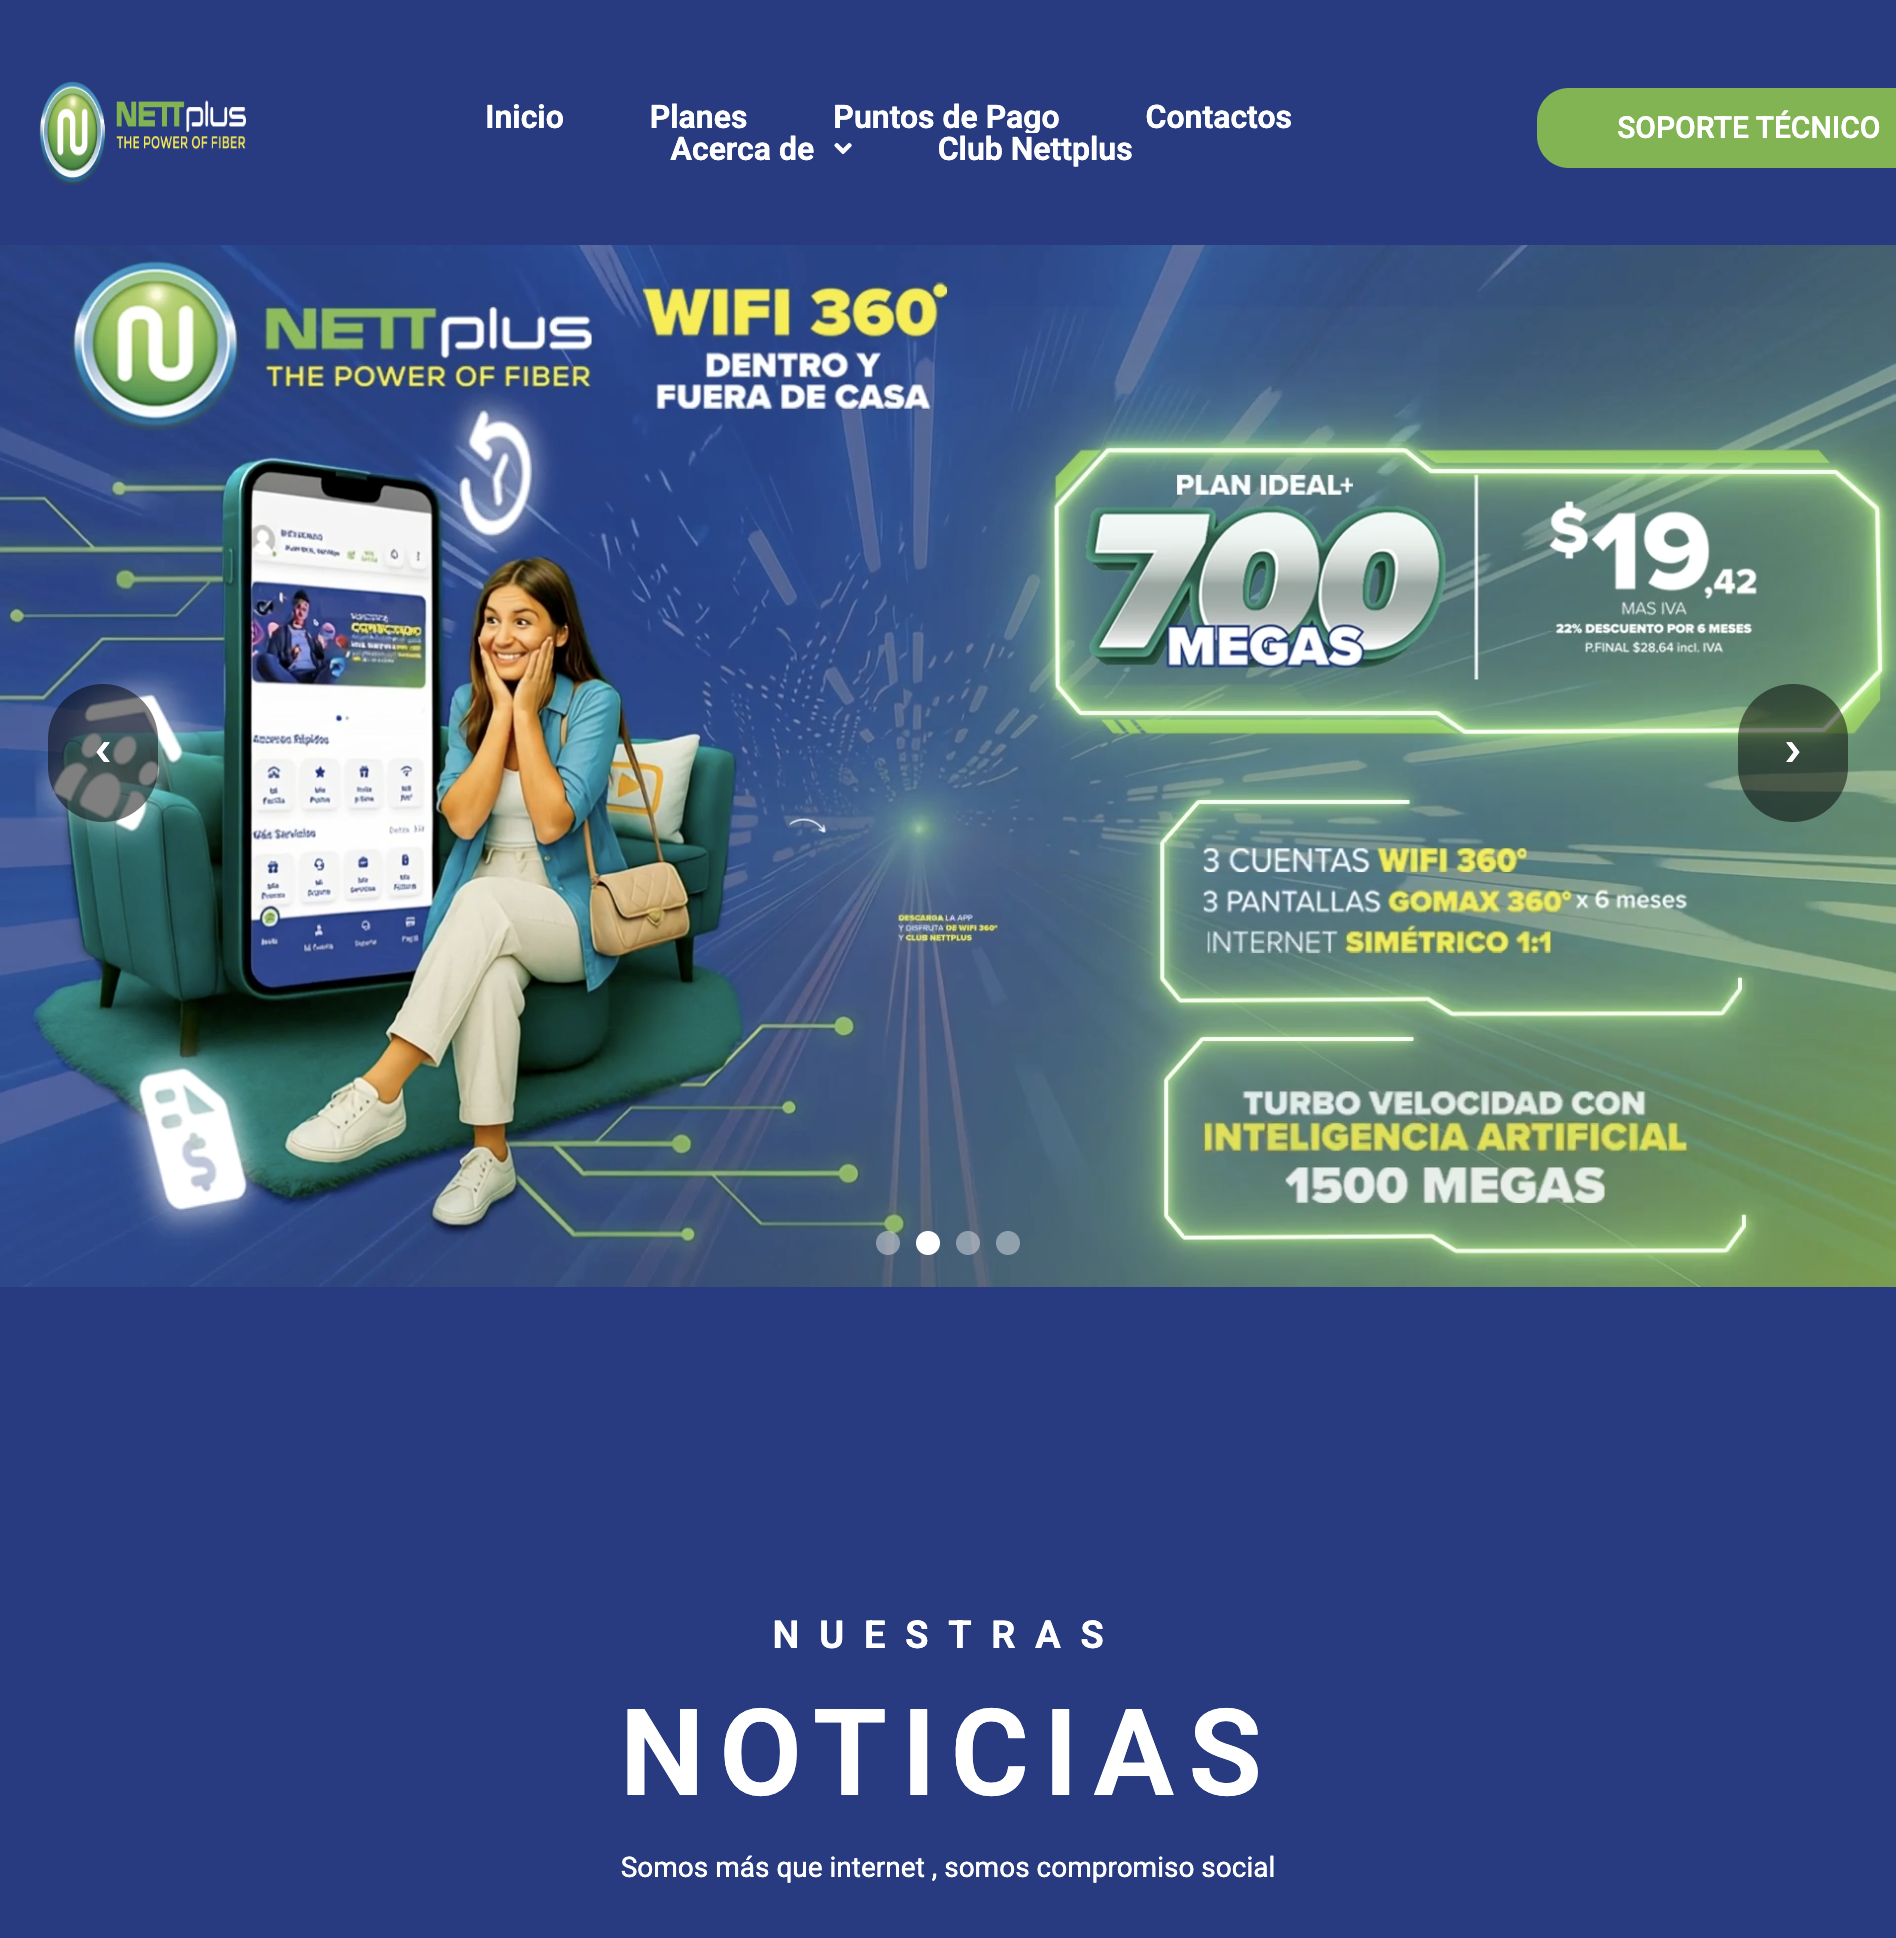
\includegraphics[width=\linewidth]{fig-web-netplus-20260505-v1.png}
  \caption{Sitio web de NETPLUS. Origen: \url{https://www.nettplus.net/}. Fecha: 2026-05-05.}
\end{figure}

\begin{figure}[h]
  \centering
  
\includegraphics[width=\linewidth]{fig-web-velocity-20260505-v1.png}
  \caption{Sitio web de Velocity. Origen: \url{https://velocity.ec/}. Fecha: 2026-05-05.}
\end{figure}

\begin{figure}[h]
  \centering
  
\includegraphics[width=\linewidth]{fig-web-celerity-20260505-v1.png}
  \caption{Sitio web de Celerity. Origen: \url{https://www.celerity.ec/}. Fecha: 2026-05-05.}
\end{figure}

\begin{figure}[h]
  \centering
  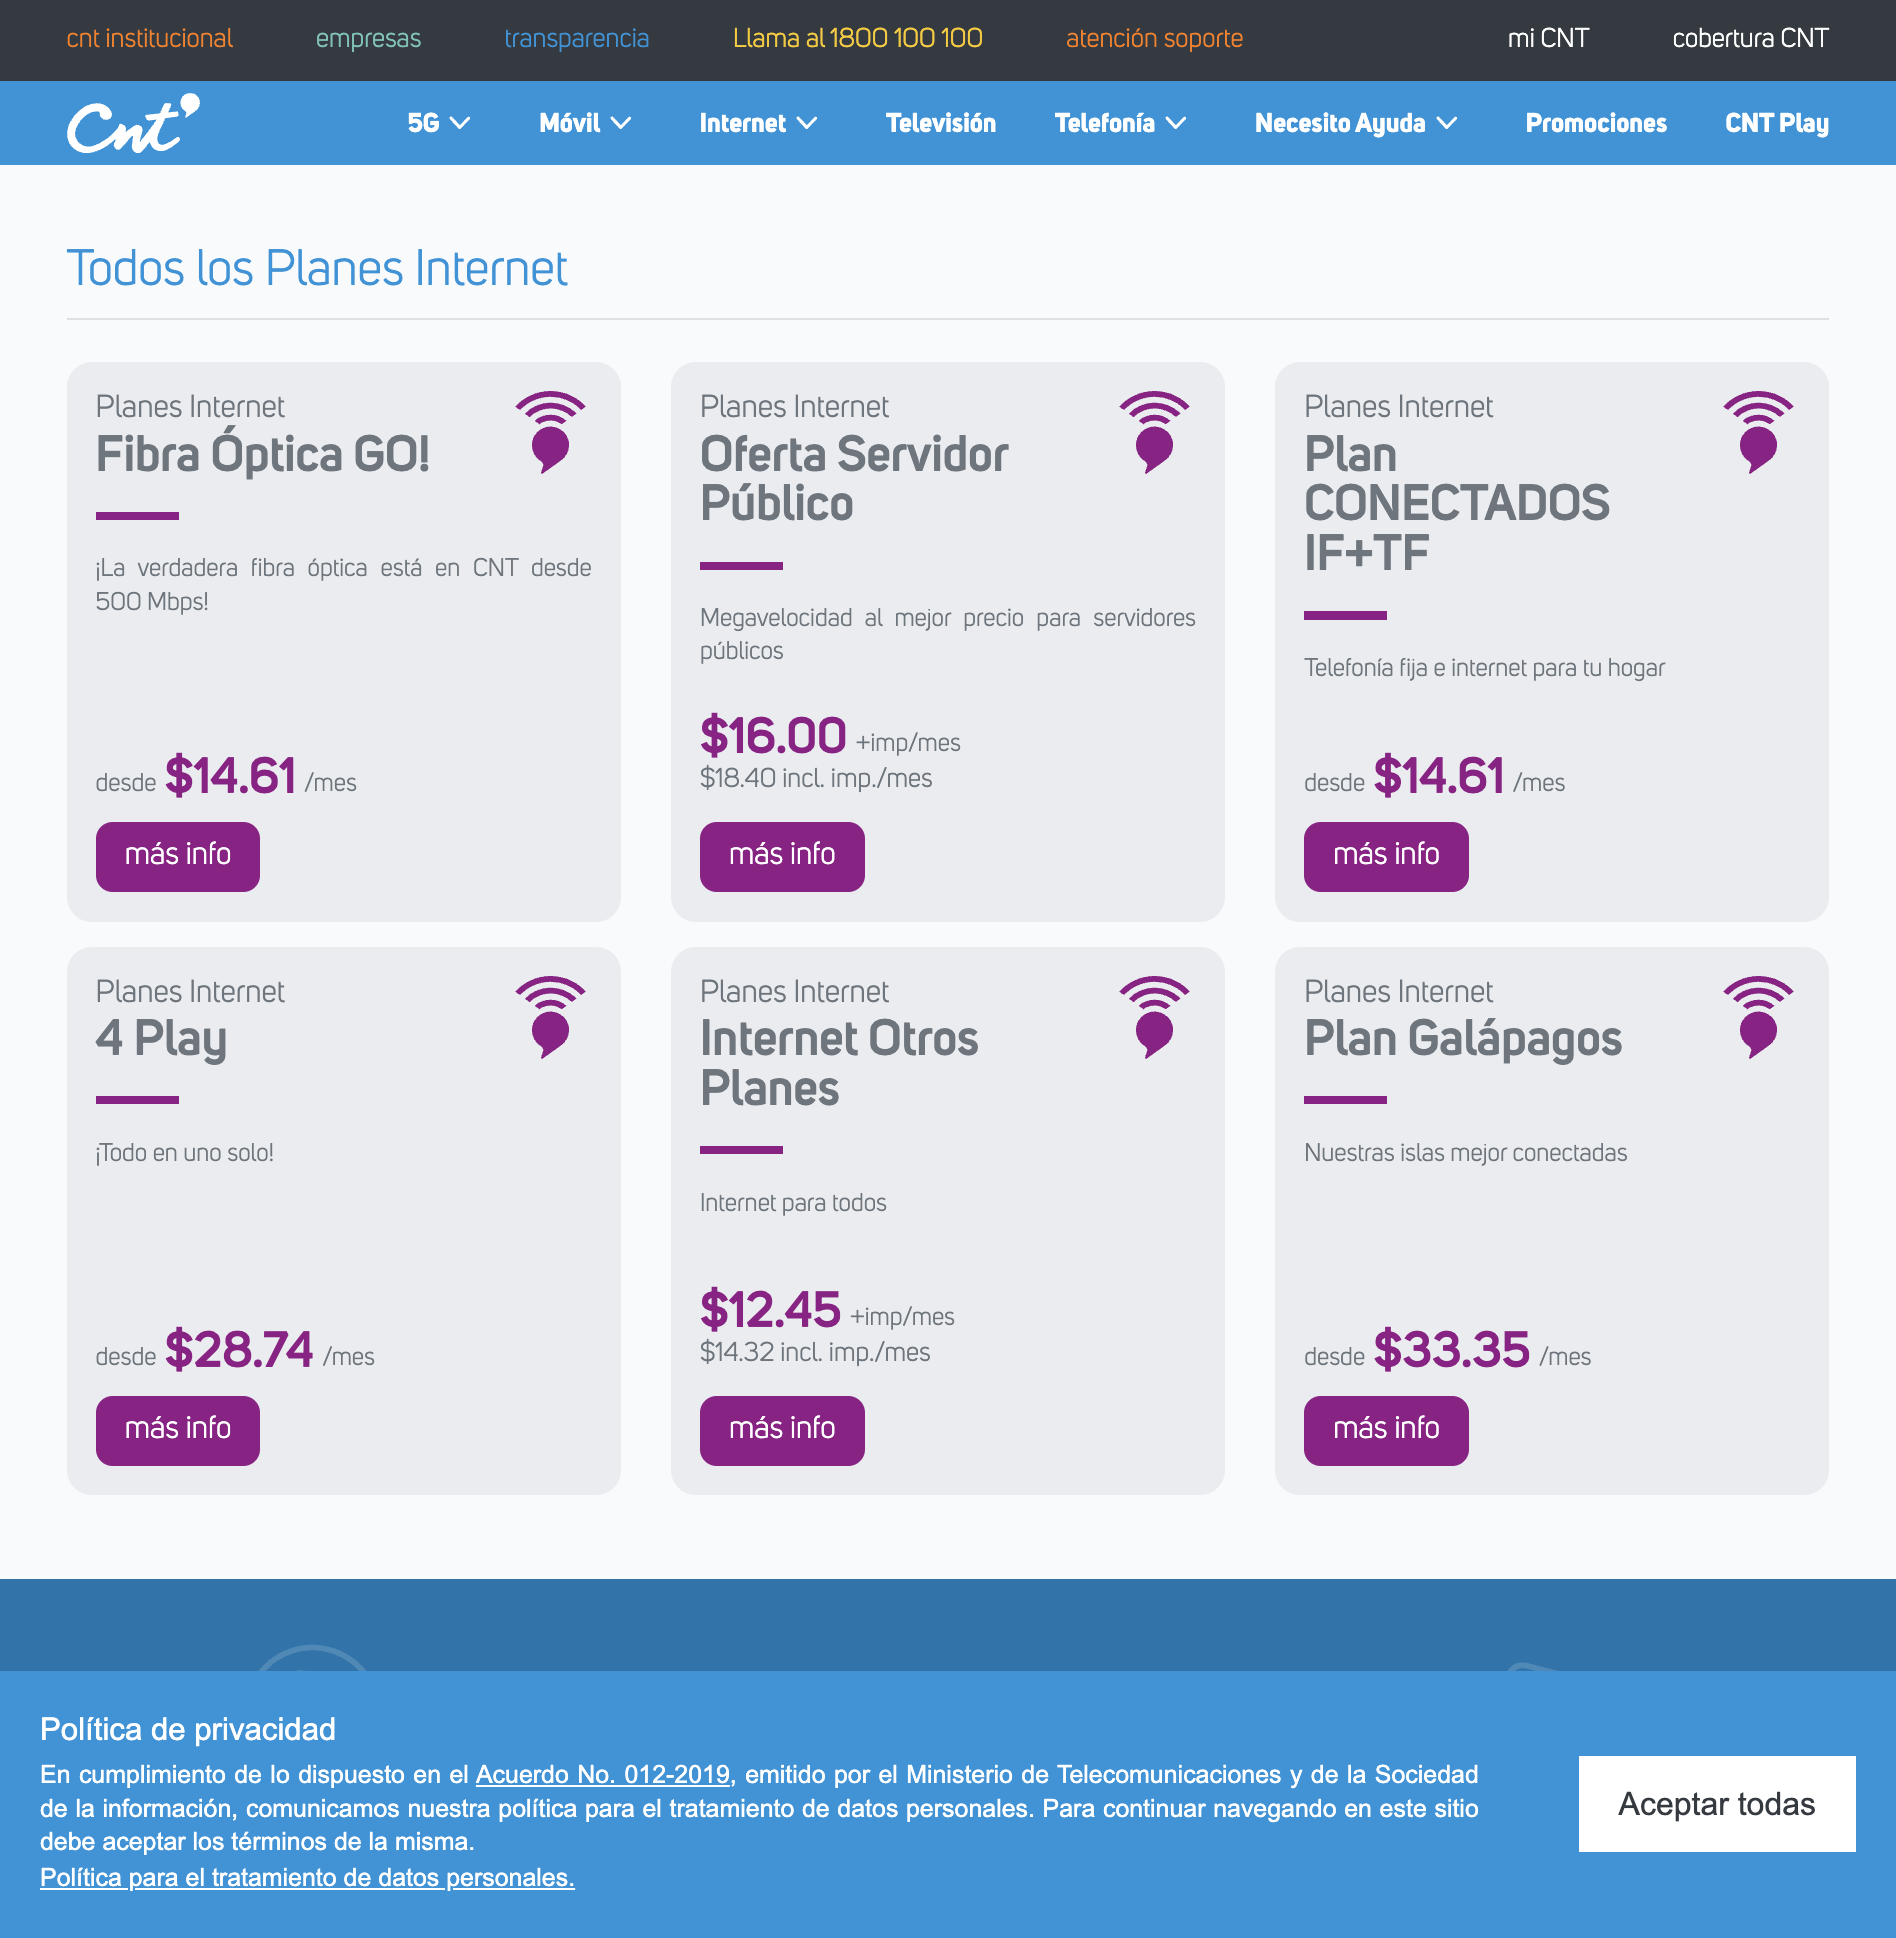
\includegraphics[width=\linewidth]{fig-web-cnt-20260505-v1.png}
  \caption{Pagina de planes CNT. Origen: \url{https://www.cnt.com.ec/productos/planes-internet}. Fecha: 2026-05-05.}
\end{figure}

\begin{figure}[h]
  \centering
  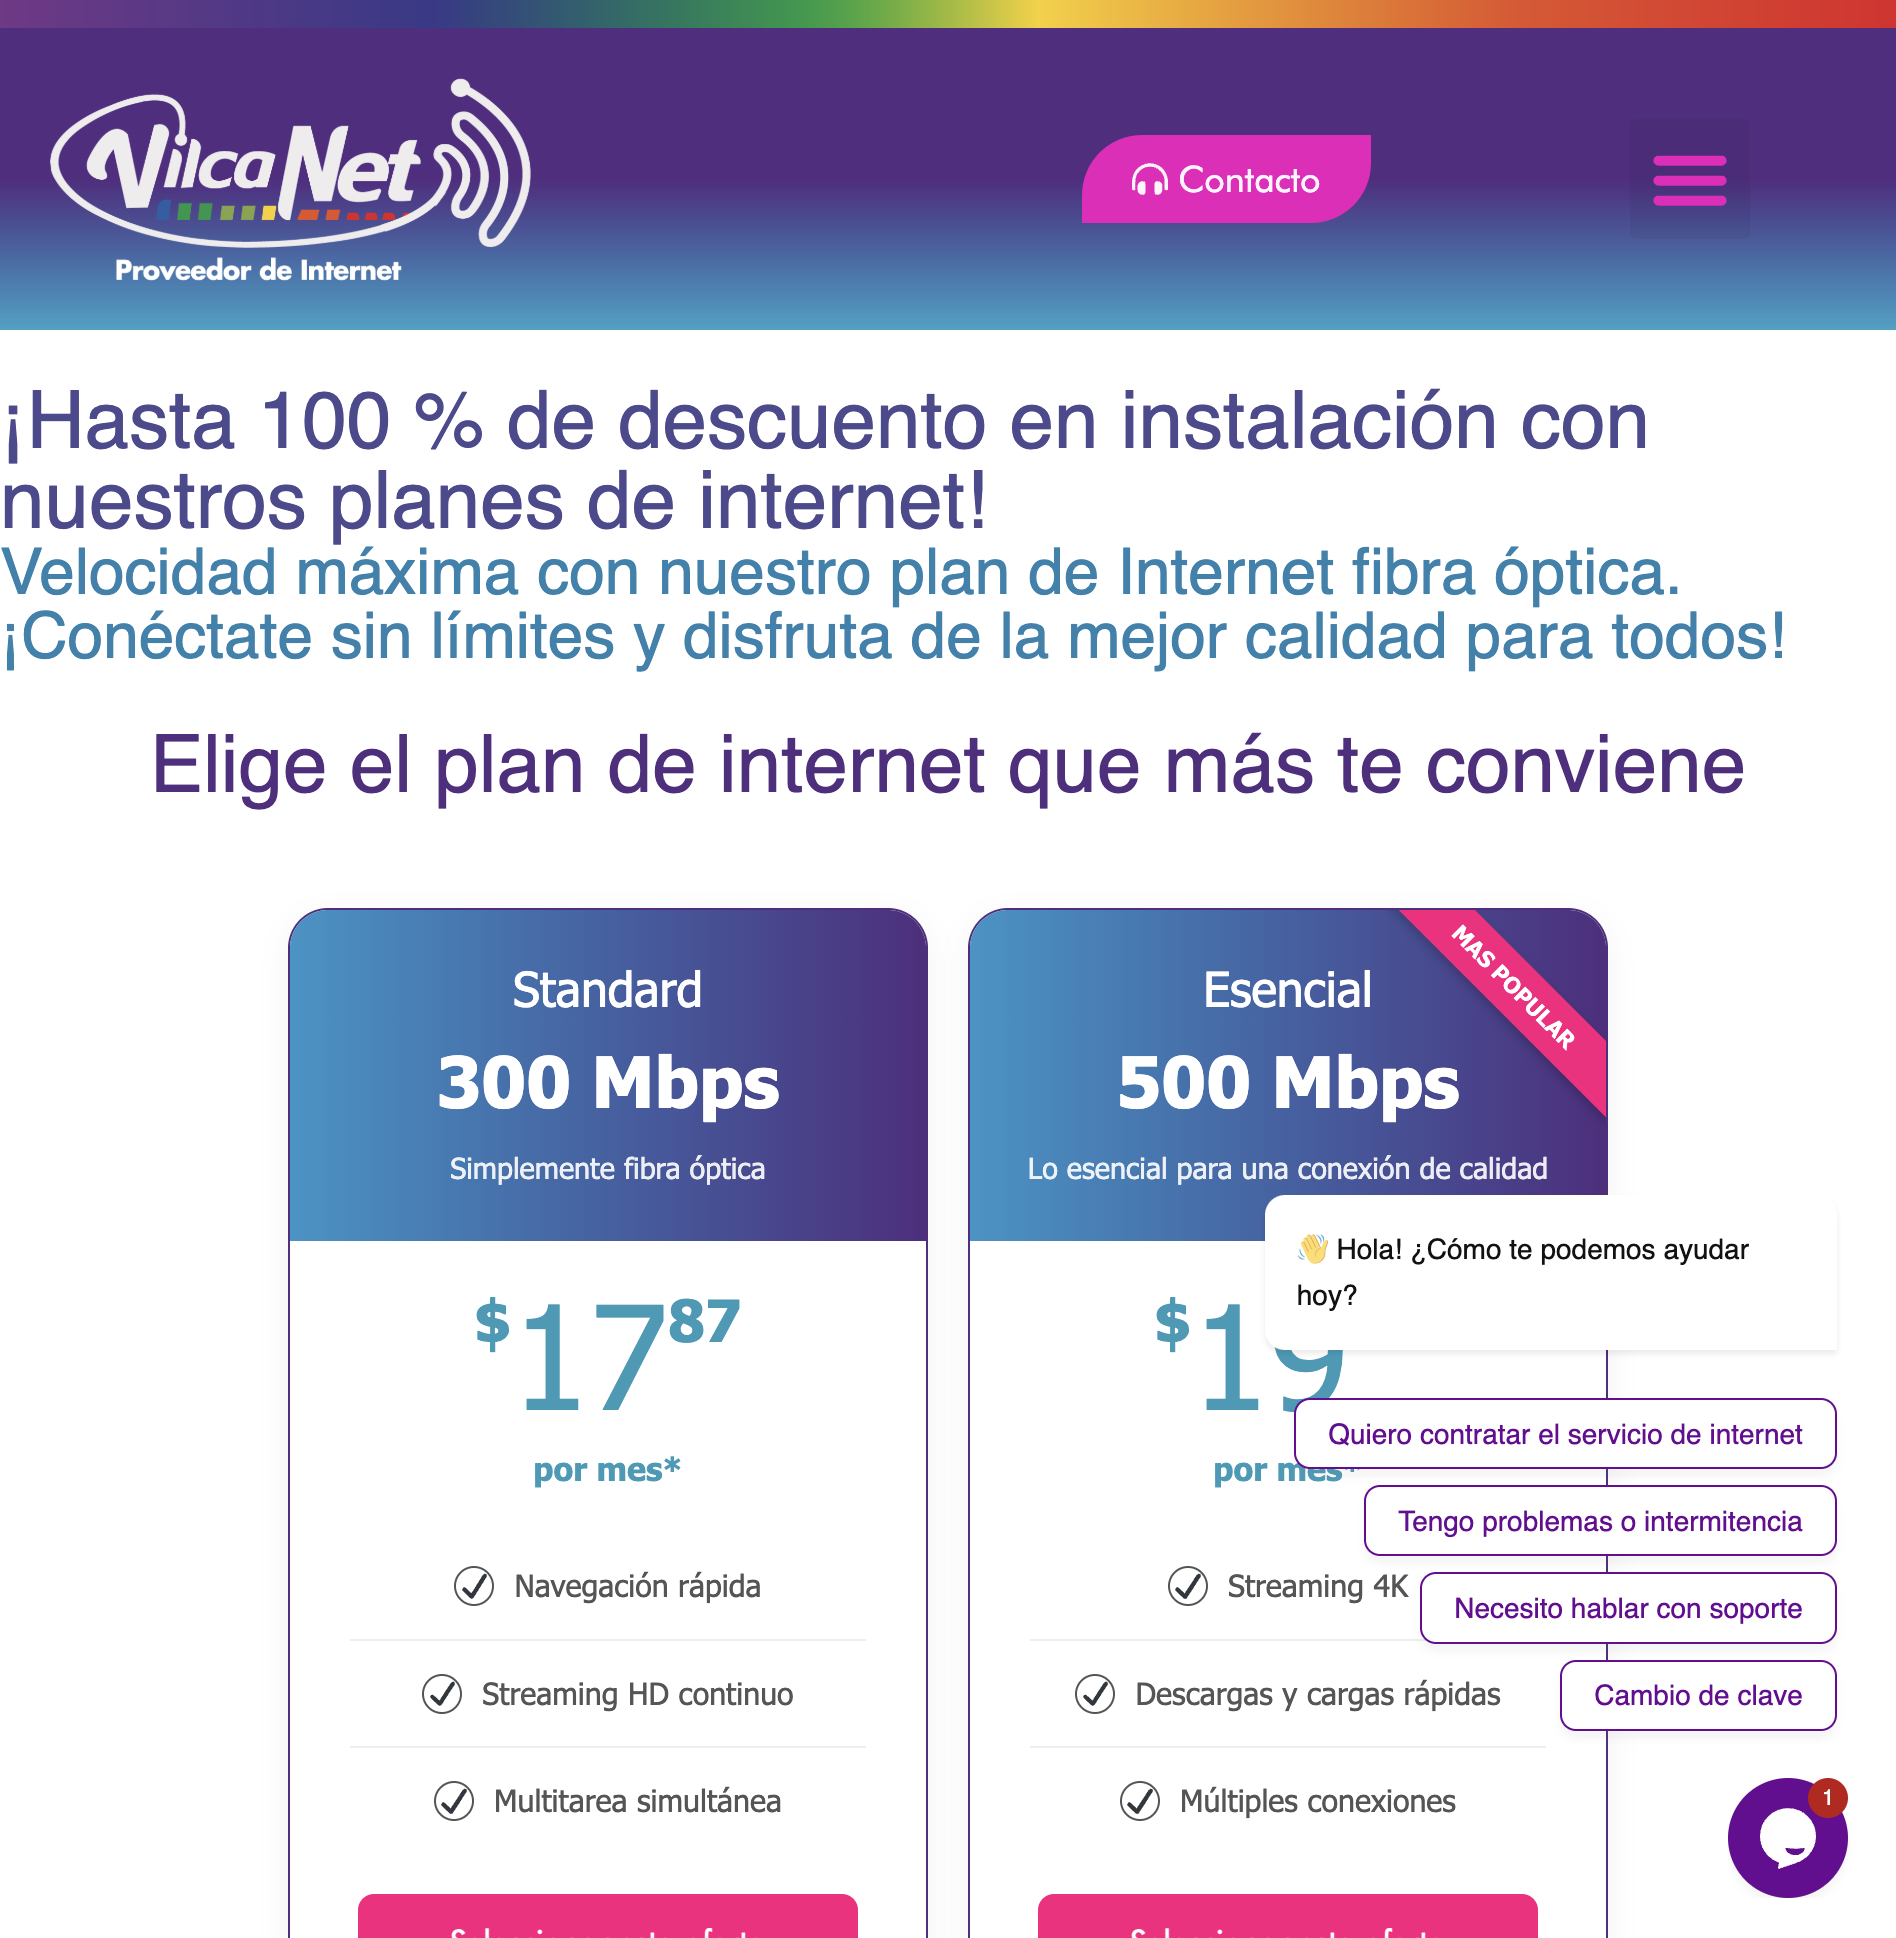
\includegraphics[width=\linewidth]{fig-web-vilcanet-20260505-v1.png}
  \caption{Sitio web de Vilcanet. Origen: \url{https://vilcanet.com/}. Fecha: 2026-05-05.}
\end{figure}

\begin{figure}[h]
  \centering
  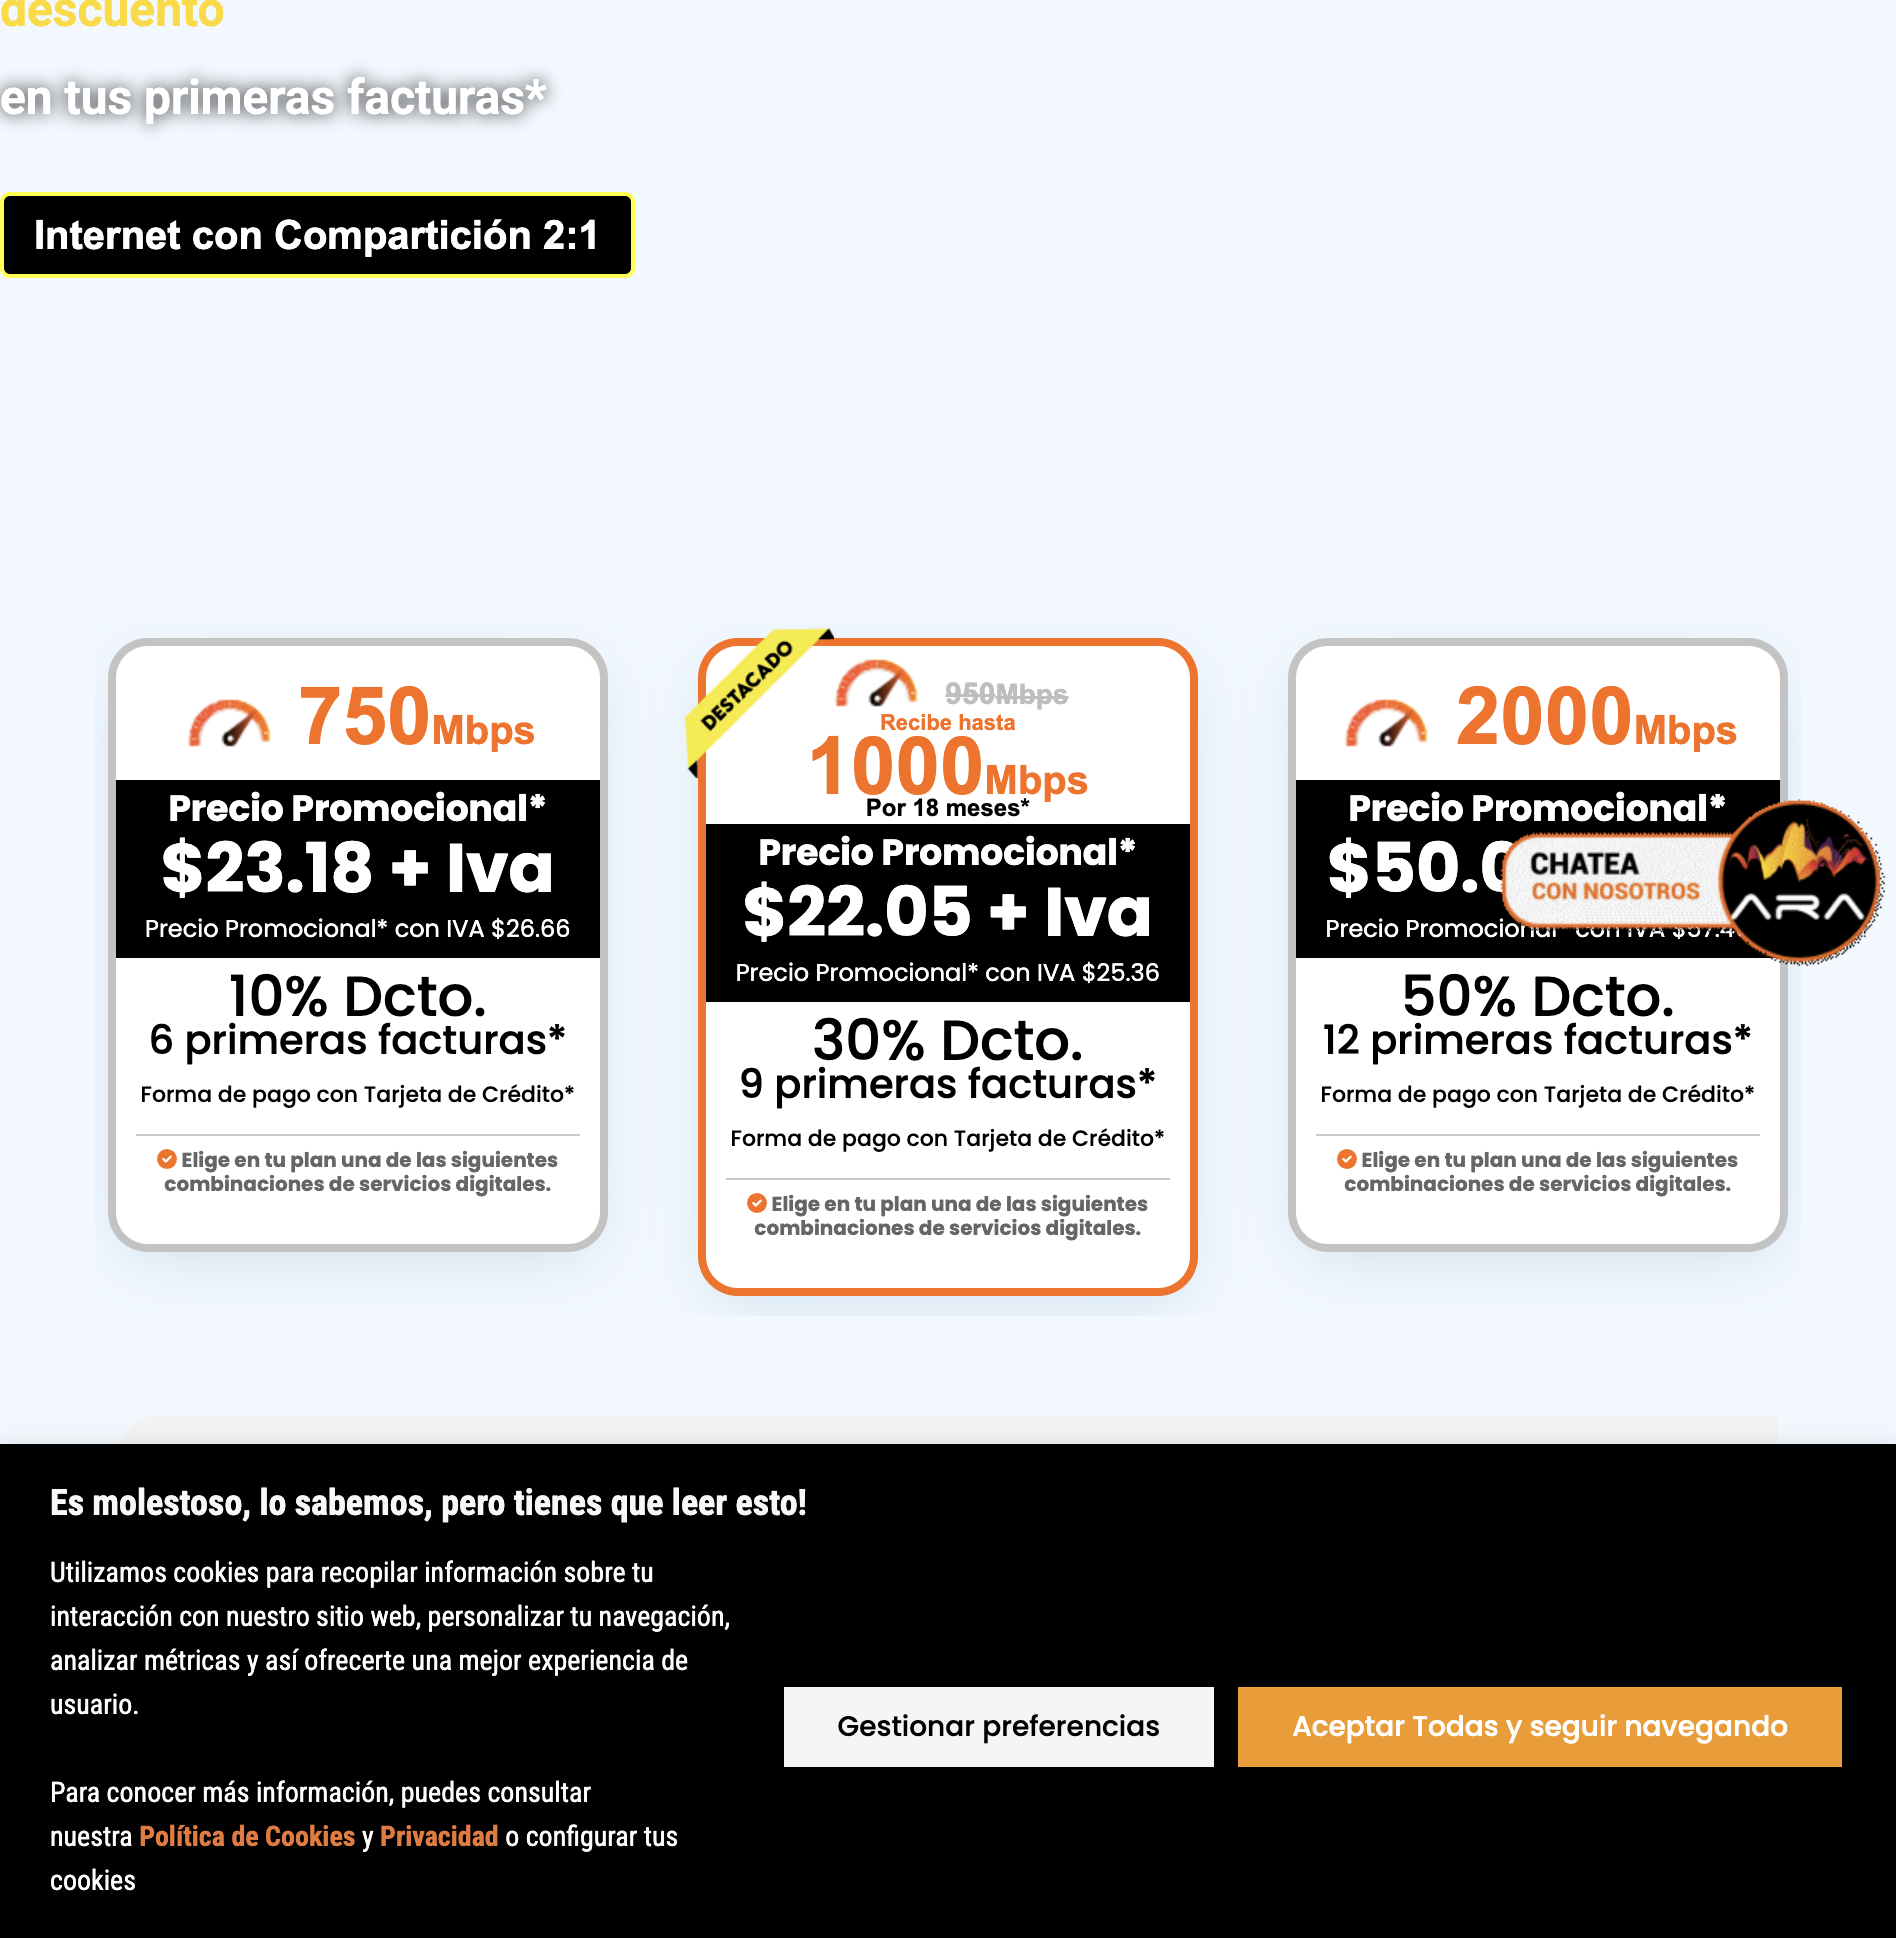
\includegraphics[width=\linewidth]{fig-web-netlife-20260505-v1.png}
  \caption{Pagina de planes Netlife. Origen: \url{https://netlife.ec/planes-hogar/}. Fecha: 2026-05-05.}
\end{figure}

\begin{figure}[h]
  \centering
  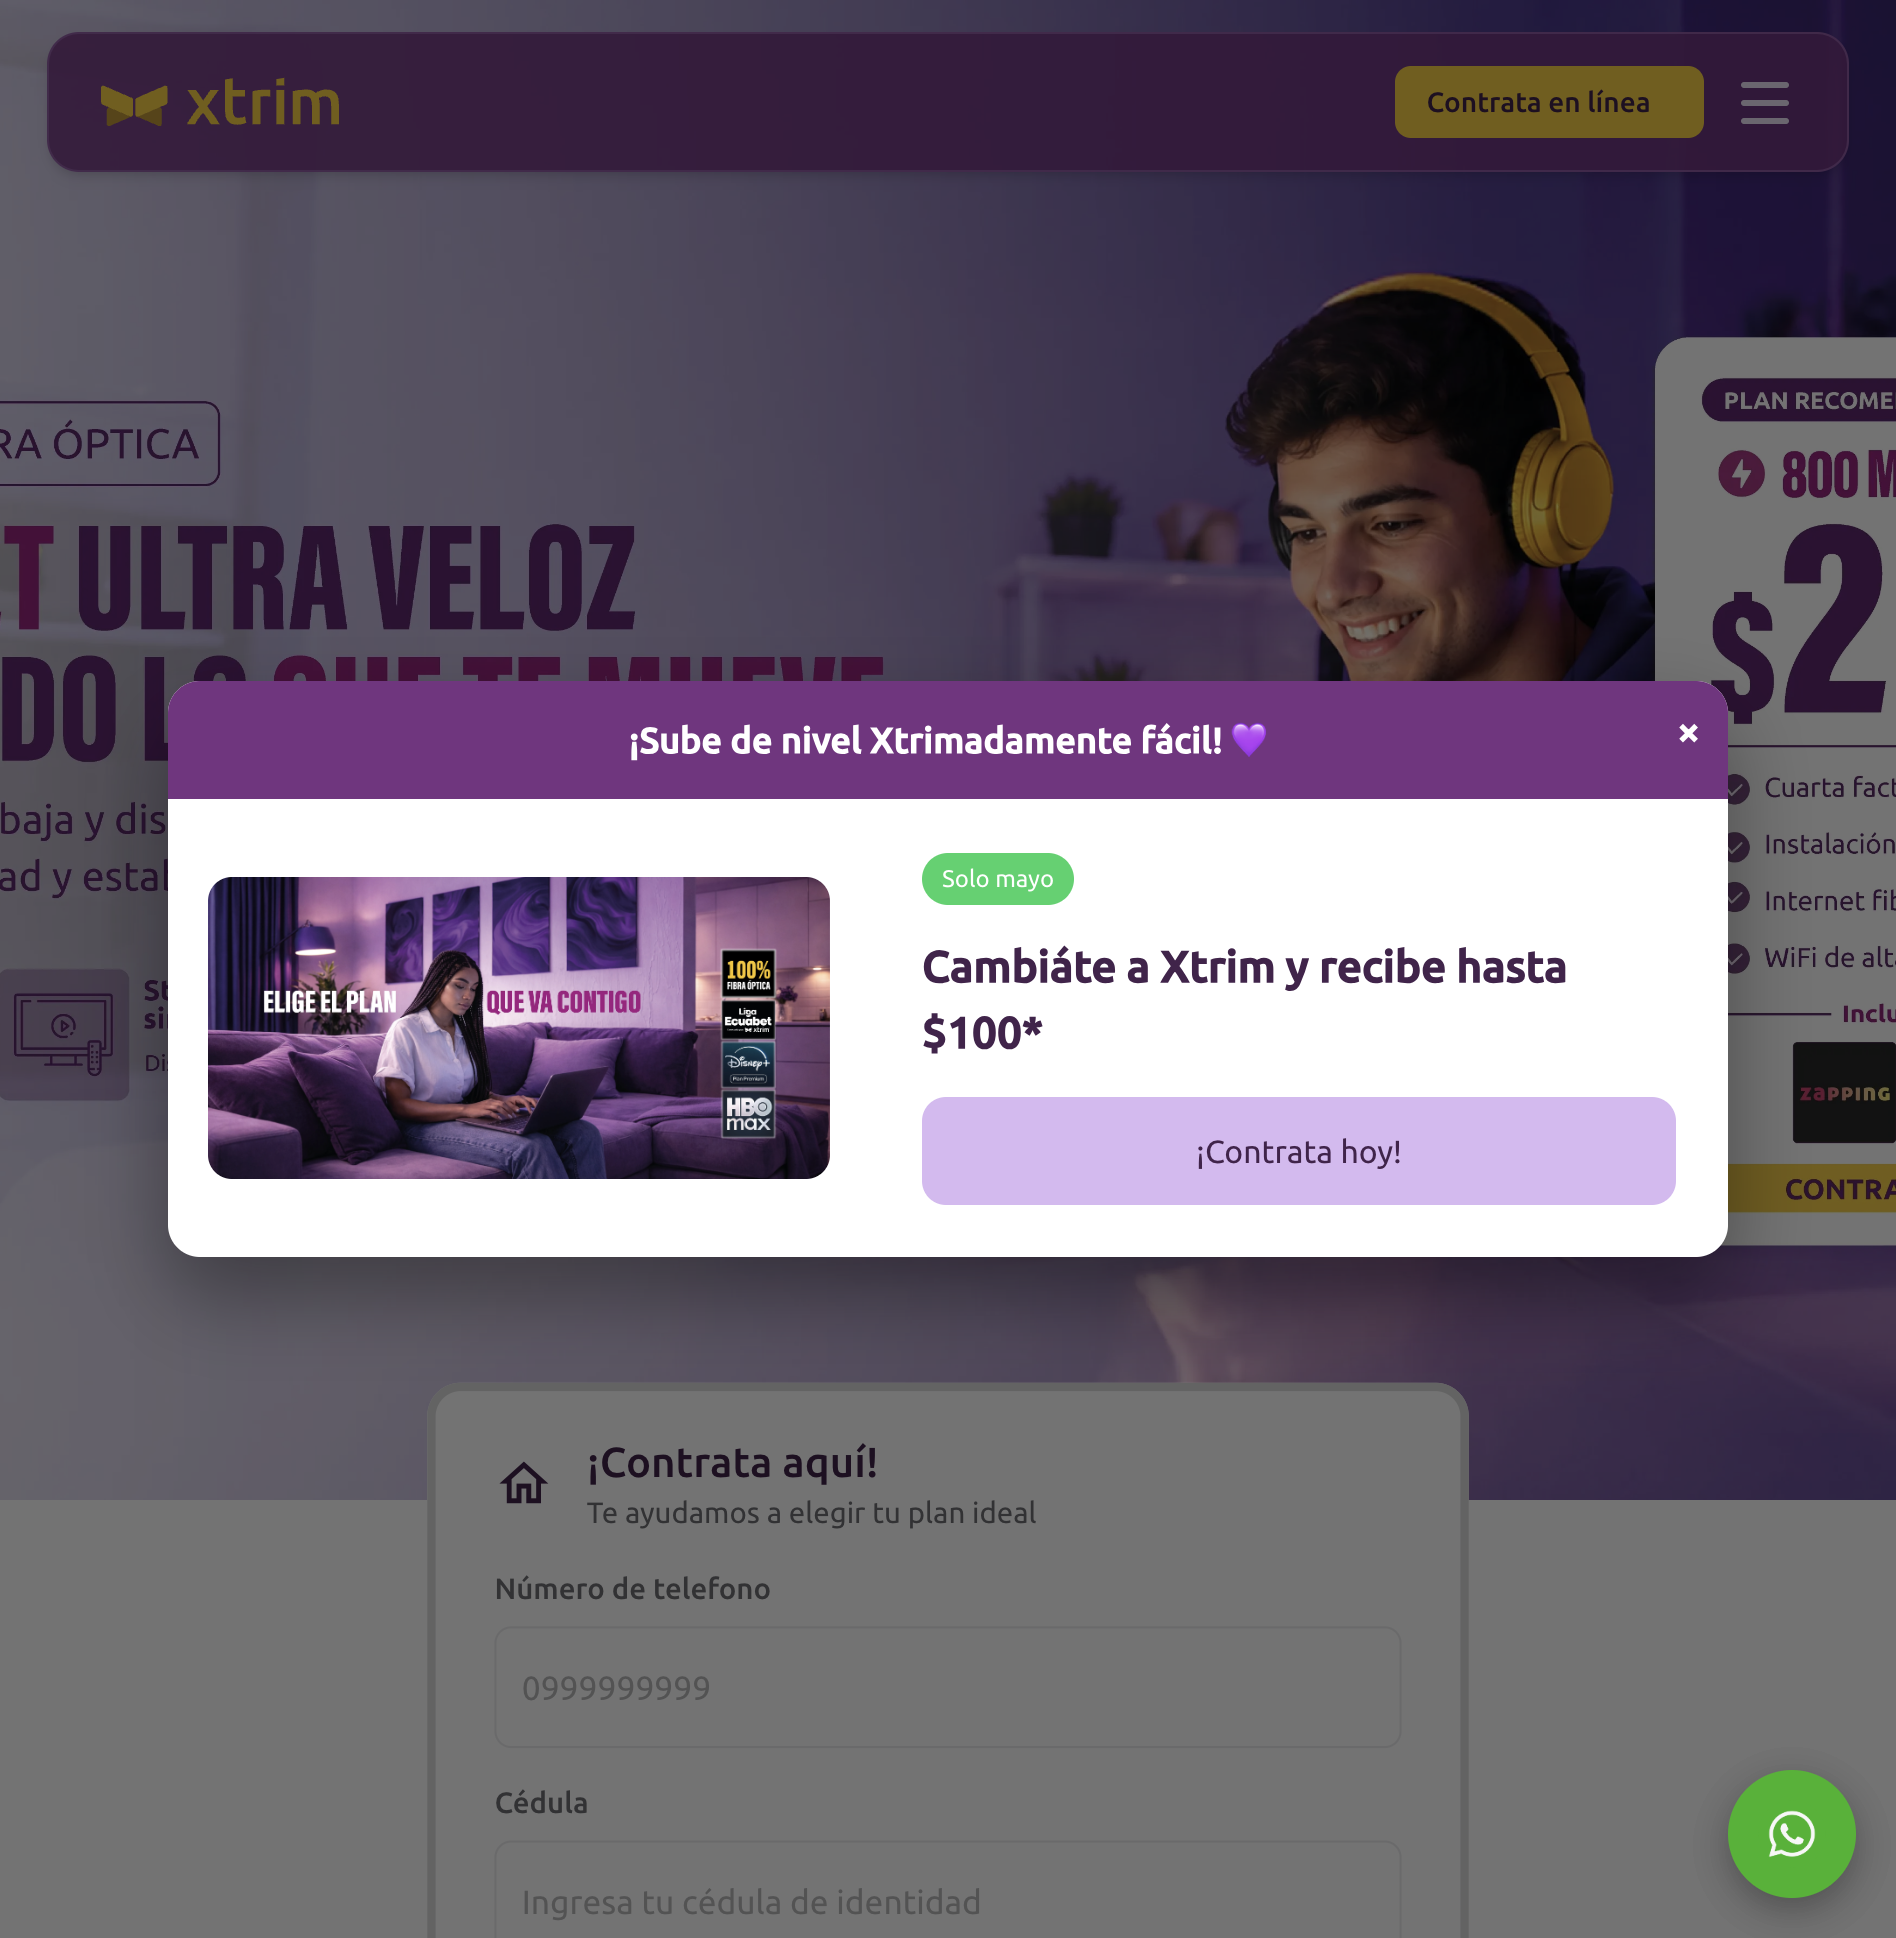
\includegraphics[width=\linewidth]{fig-web-xtrim-20260505-v1.png}
  \caption{Pagina comercial Xtrim. Origen: \url{https://www.xtrim.com.ec/internet}. Fecha: 2026-05-05.}
\end{figure}

\begin{figure}[h]
  \centering
  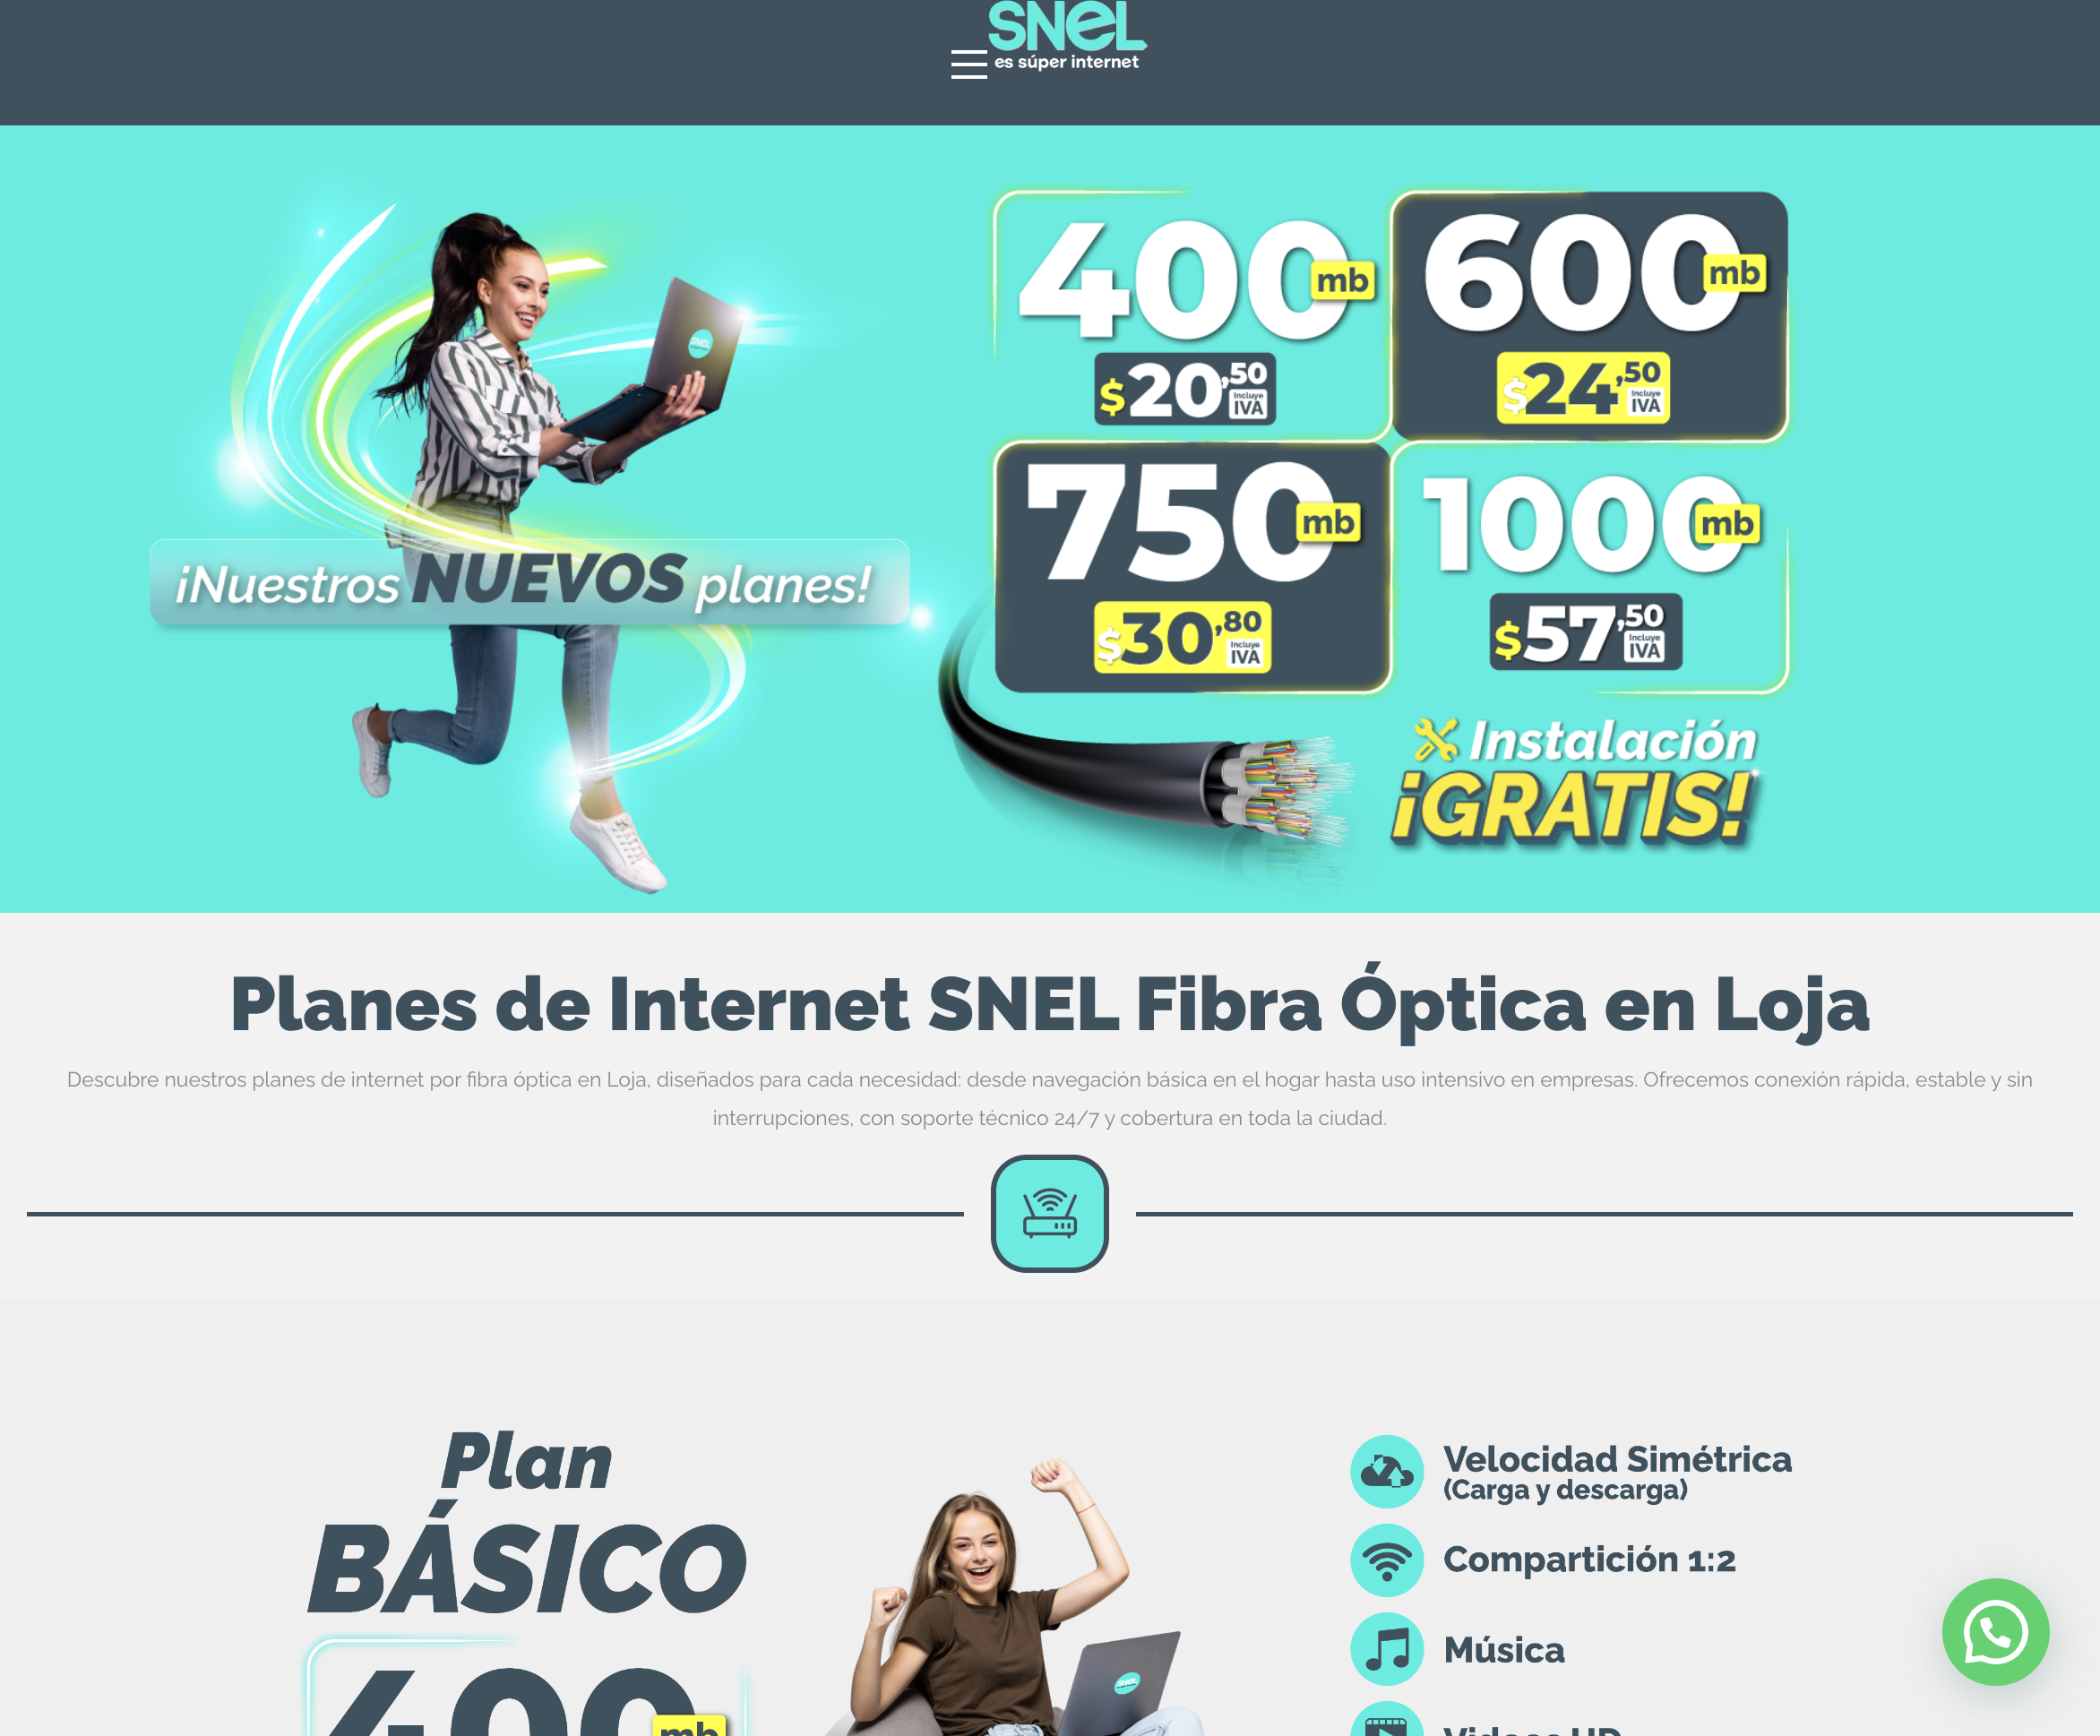
\includegraphics[width=\linewidth]{fig-web-snel-20260505-v1.png}
  \caption{Pagina de planes Snel. Origen: \url{https://etelnetsol.com/planes-2025/}. Fecha: 2026-05-05.}
\end{figure}

\begin{figure}[h]
  \centering
  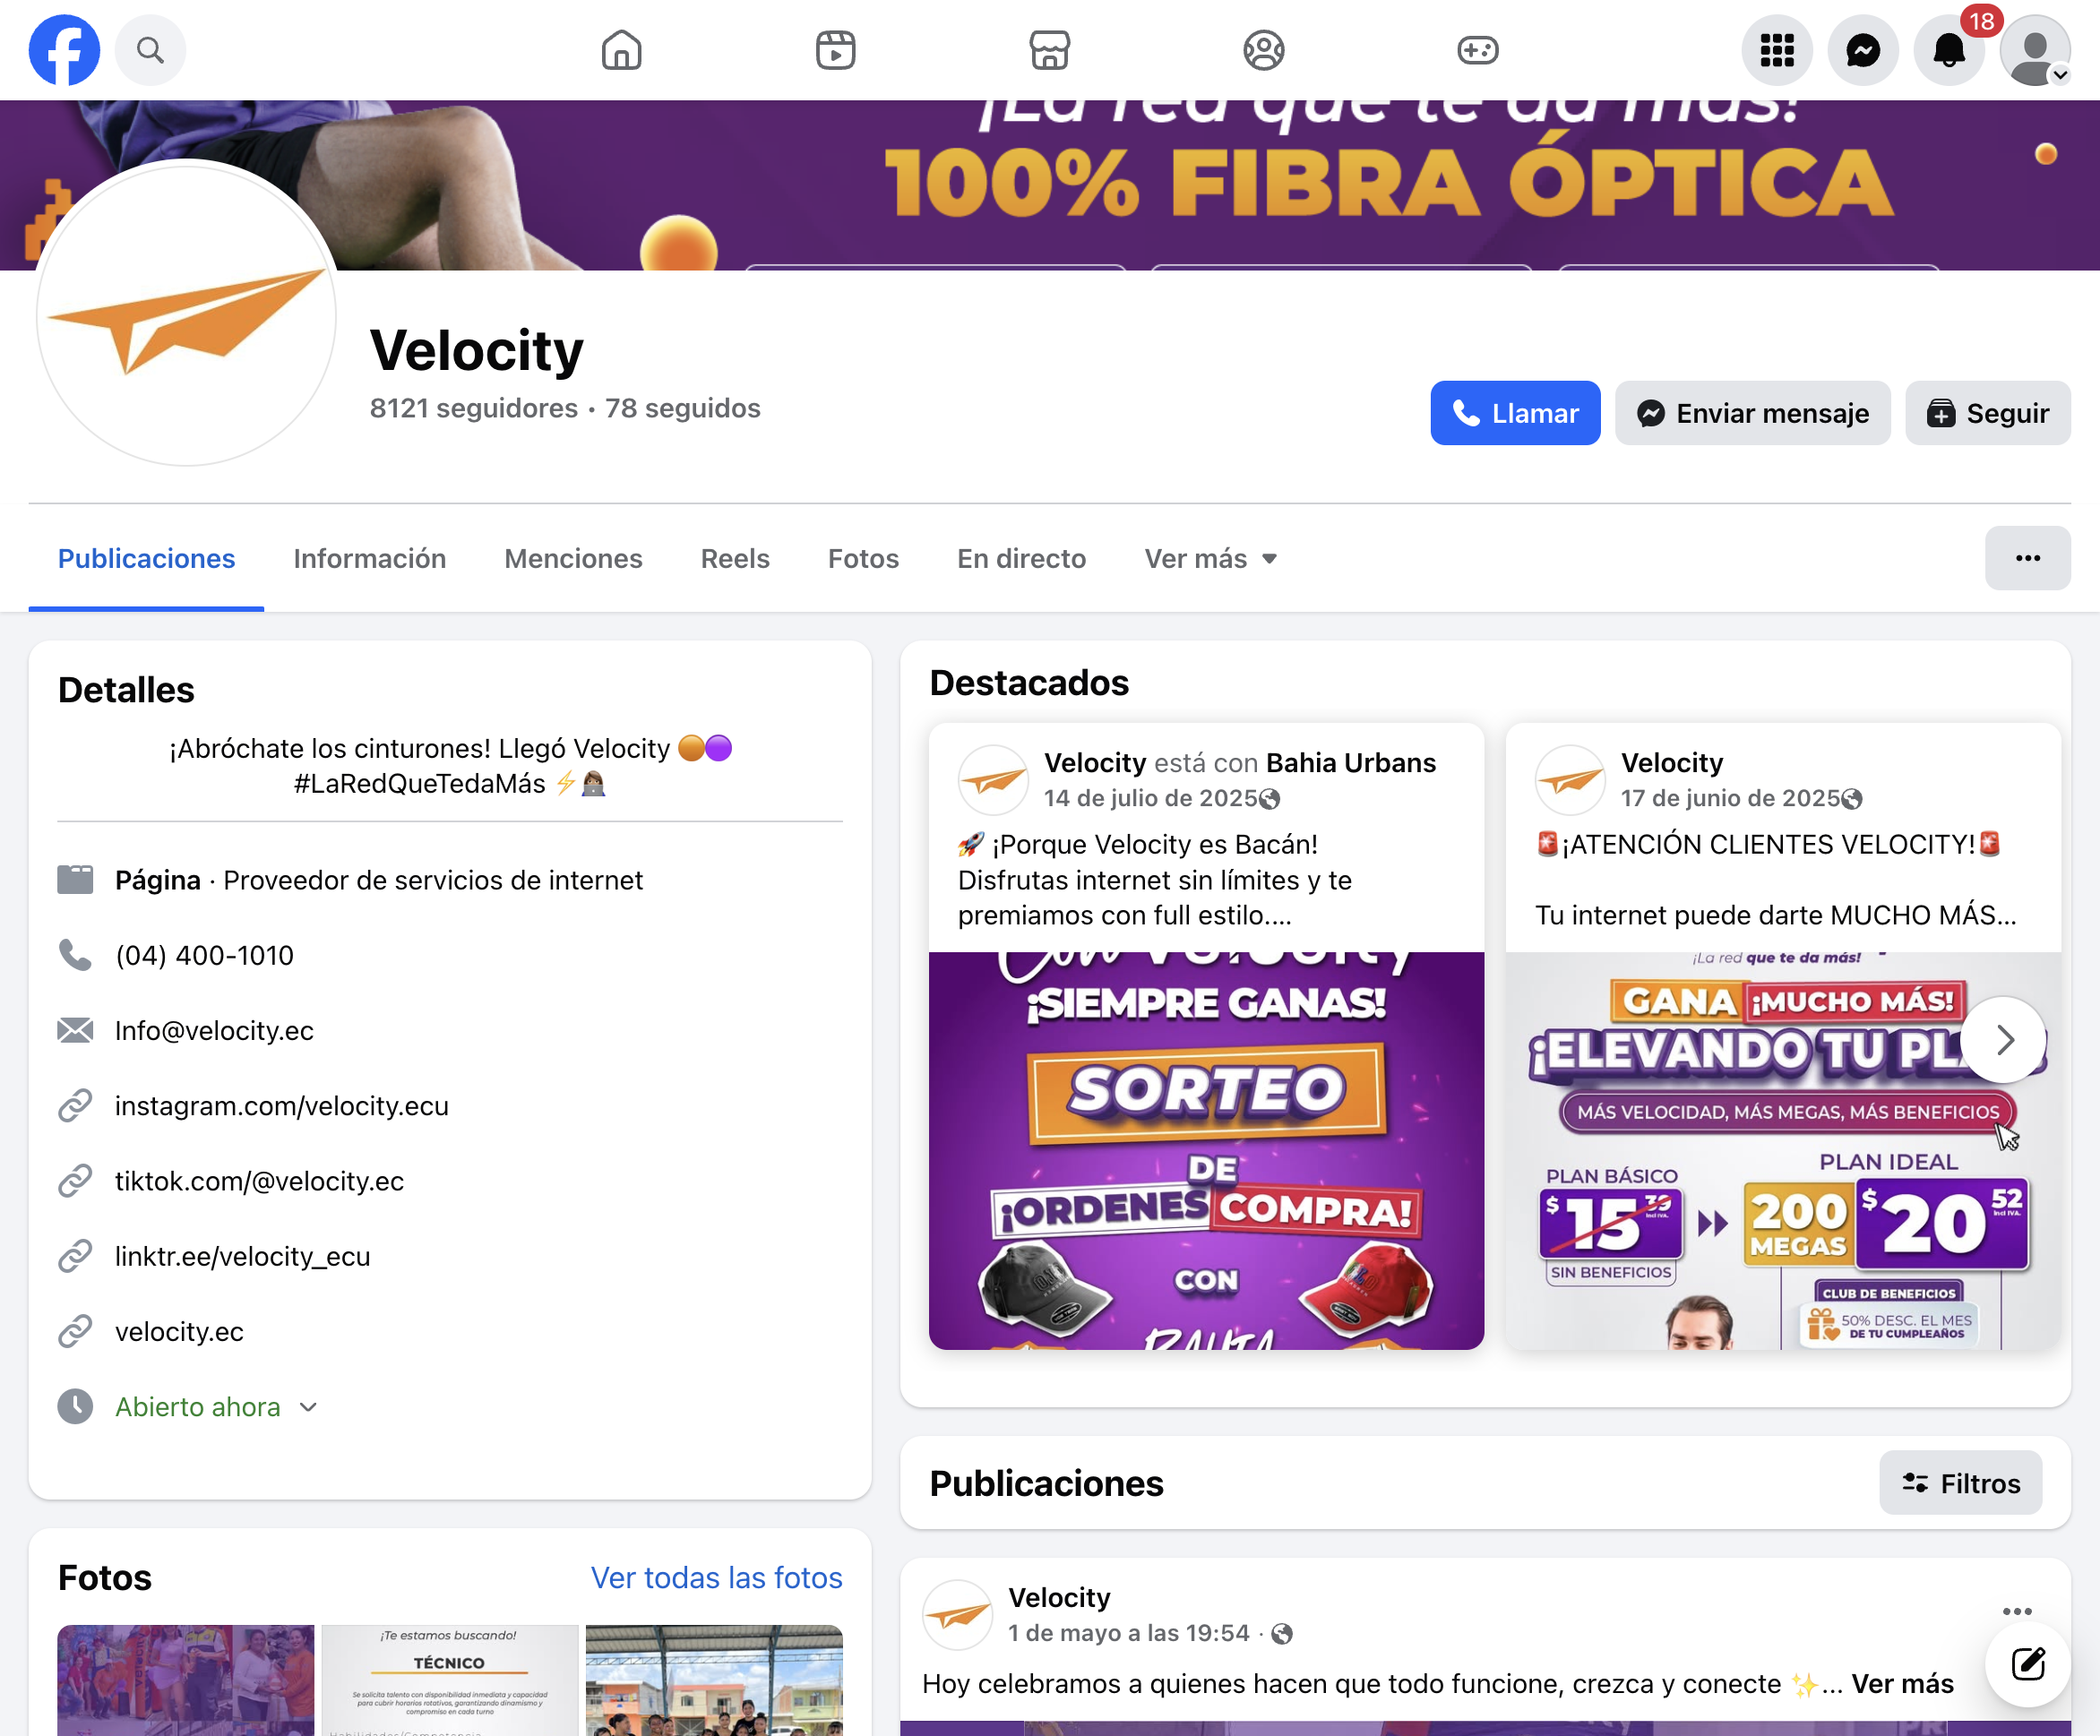
\includegraphics[width=\linewidth]{fig-facebook-velocity-20260505-v1.png}
  \caption{Facebook de Velocity. Origen: \url{https://www.facebook.com/velocity.ec/}. Fecha: 2026-05-05.}
\end{figure}

\begin{figure}[h]
  \centering
  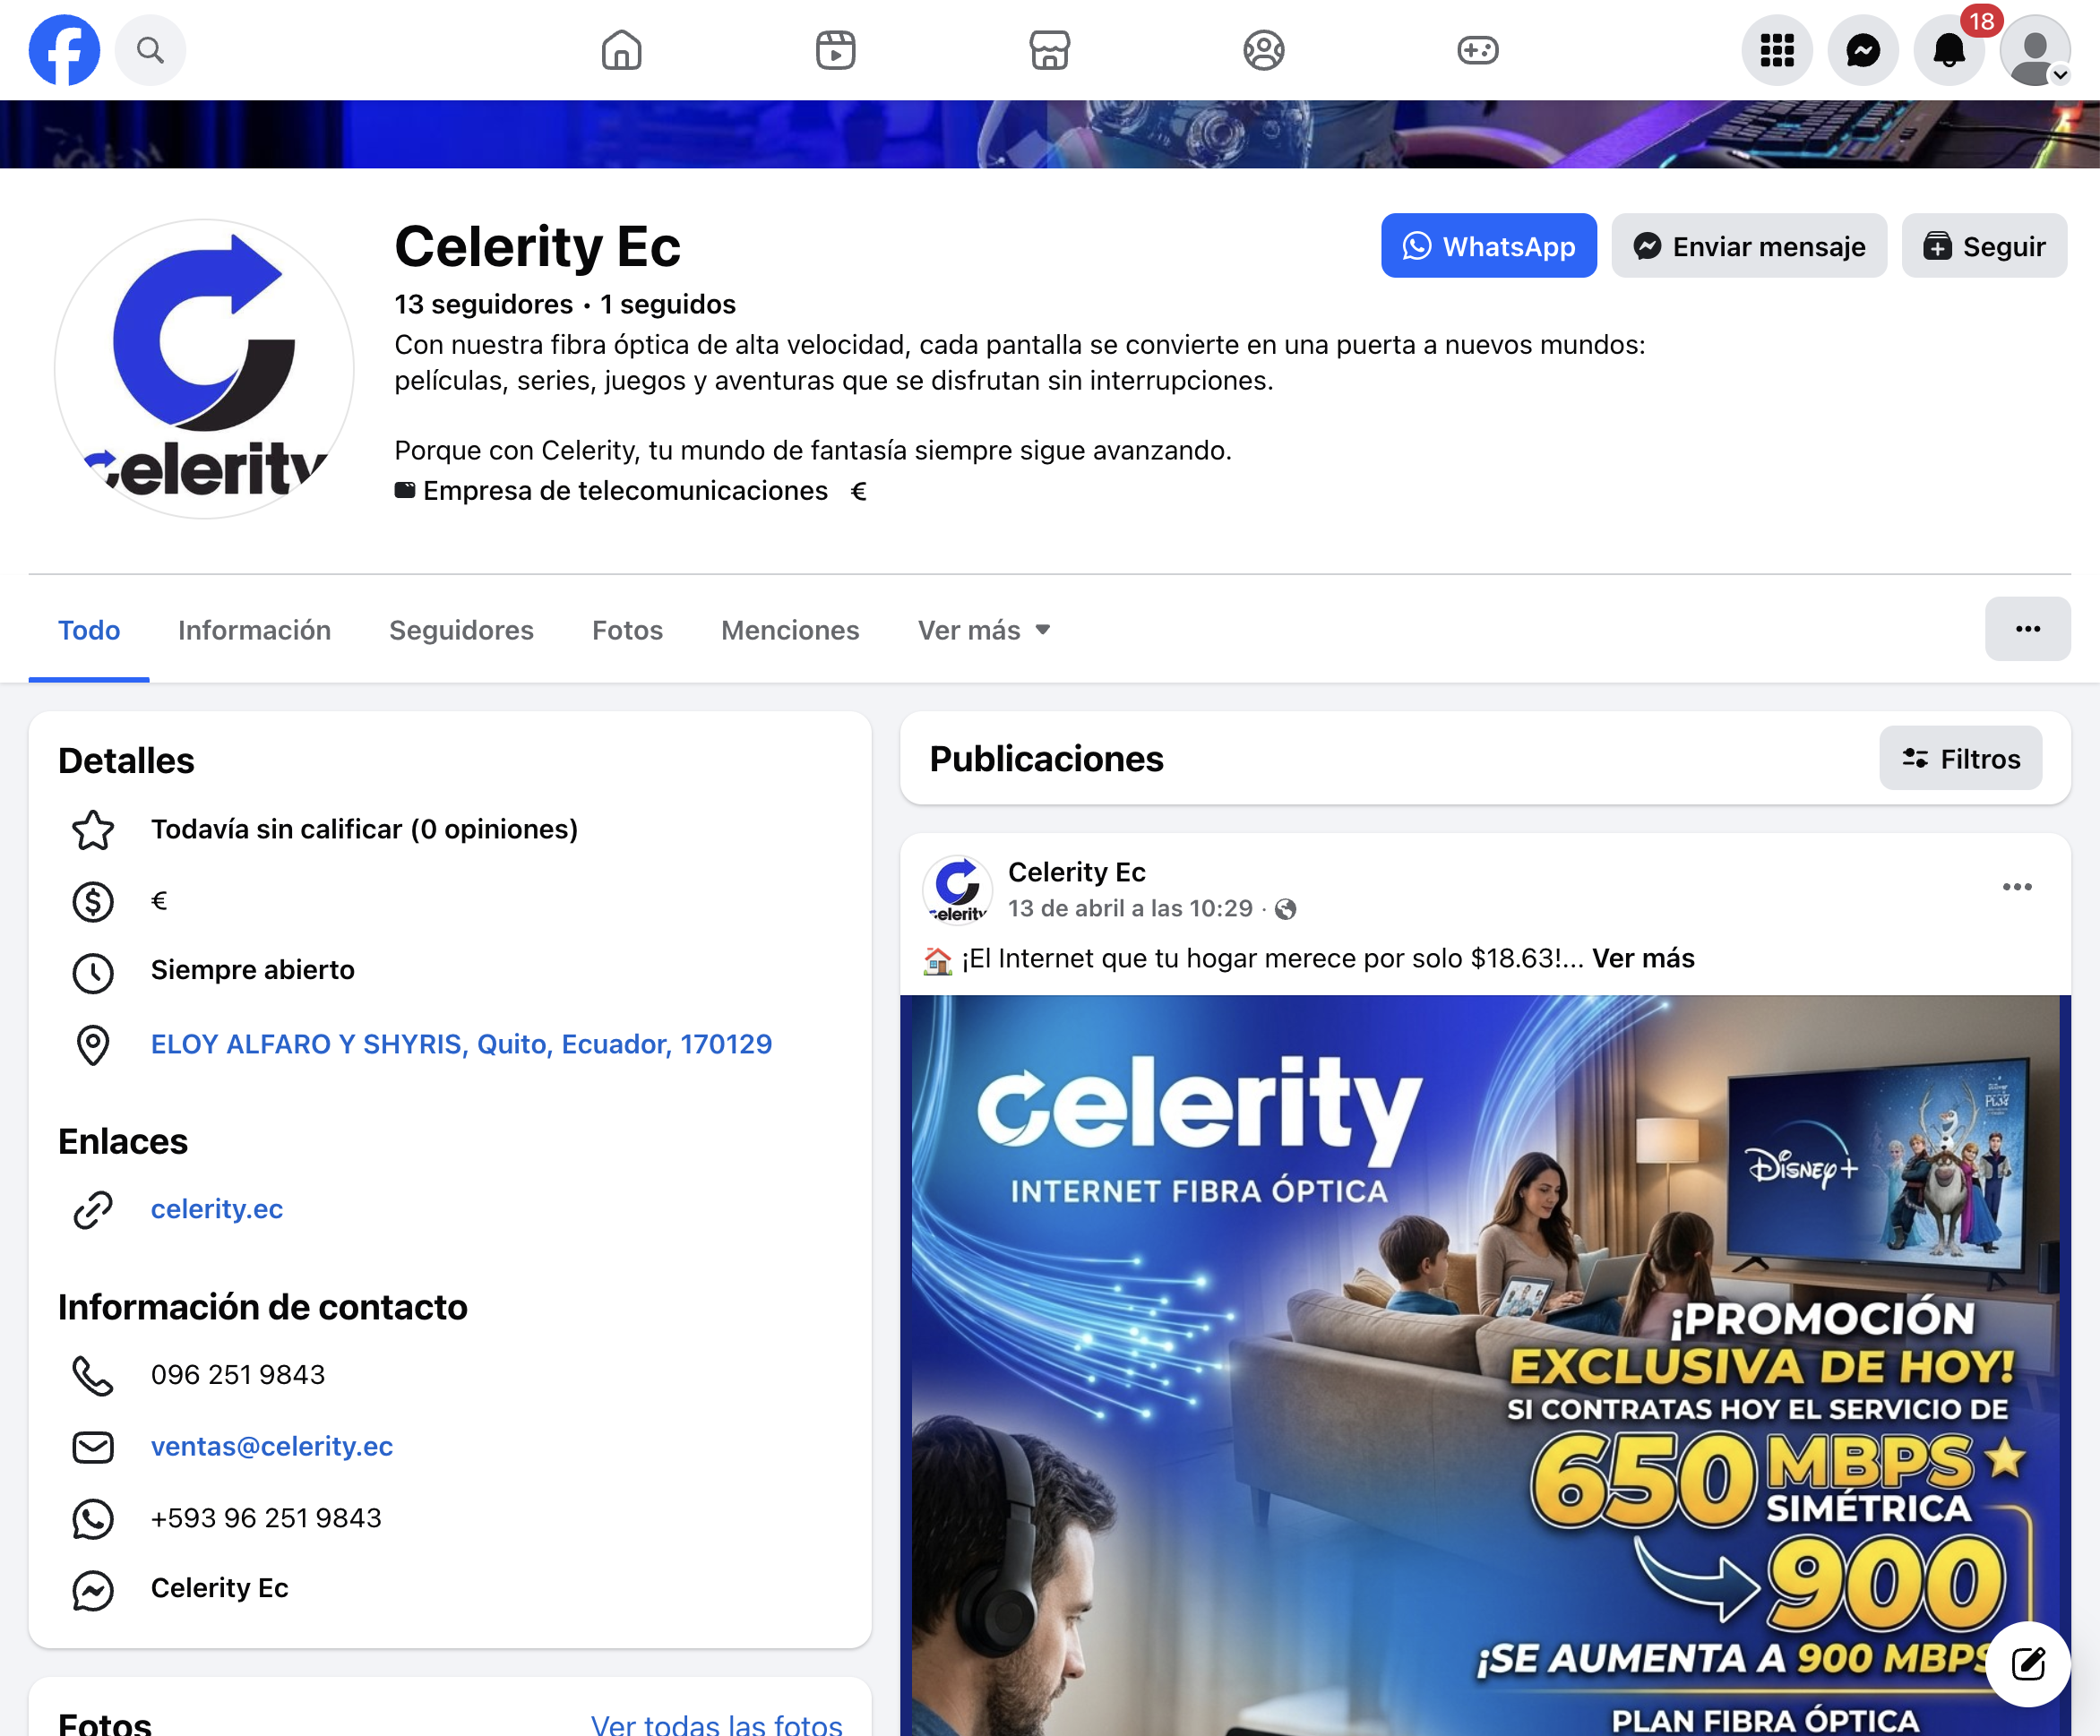
\includegraphics[width=\linewidth]{fig-facebook-celerity-20260505-v1.png}
  \caption{Facebook de Celerity (perfil evaluado). Origen: \url{https://www.facebook.com/celerityec/}. Fecha: 2026-05-05.}
\end{figure}

\begin{figure}[h]
  \centering
  
\includegraphics[width=\linewidth]{fig-facebook-cnt-20260505-v1.png}
  \caption{Facebook de CNT Ecuador. Origen: \url{https://www.facebook.com/CNTEcuador/}. Fecha: 2026-05-05.}
\end{figure}

\begin{figure}[h]
  \centering
  
\includegraphics[width=\linewidth]{fig-facebook-vilcanet-20260505-v1.png}
  \caption{Facebook de Vilcanet. Origen: \url{https://www.facebook.com/vilcanet/}. Fecha: 2026-05-05.}
\end{figure}

\begin{figure}[h]
  \centering
  
\includegraphics[width=\linewidth]{fig-facebook-xtrim-20260505-v1.png}
  \caption{Facebook de Xtrim Ecuador. Origen: \url{https://www.facebook.com/xtrimecuador/}. Fecha: 2026-05-05.}
\end{figure}

\begin{figure}[h]
  \centering
  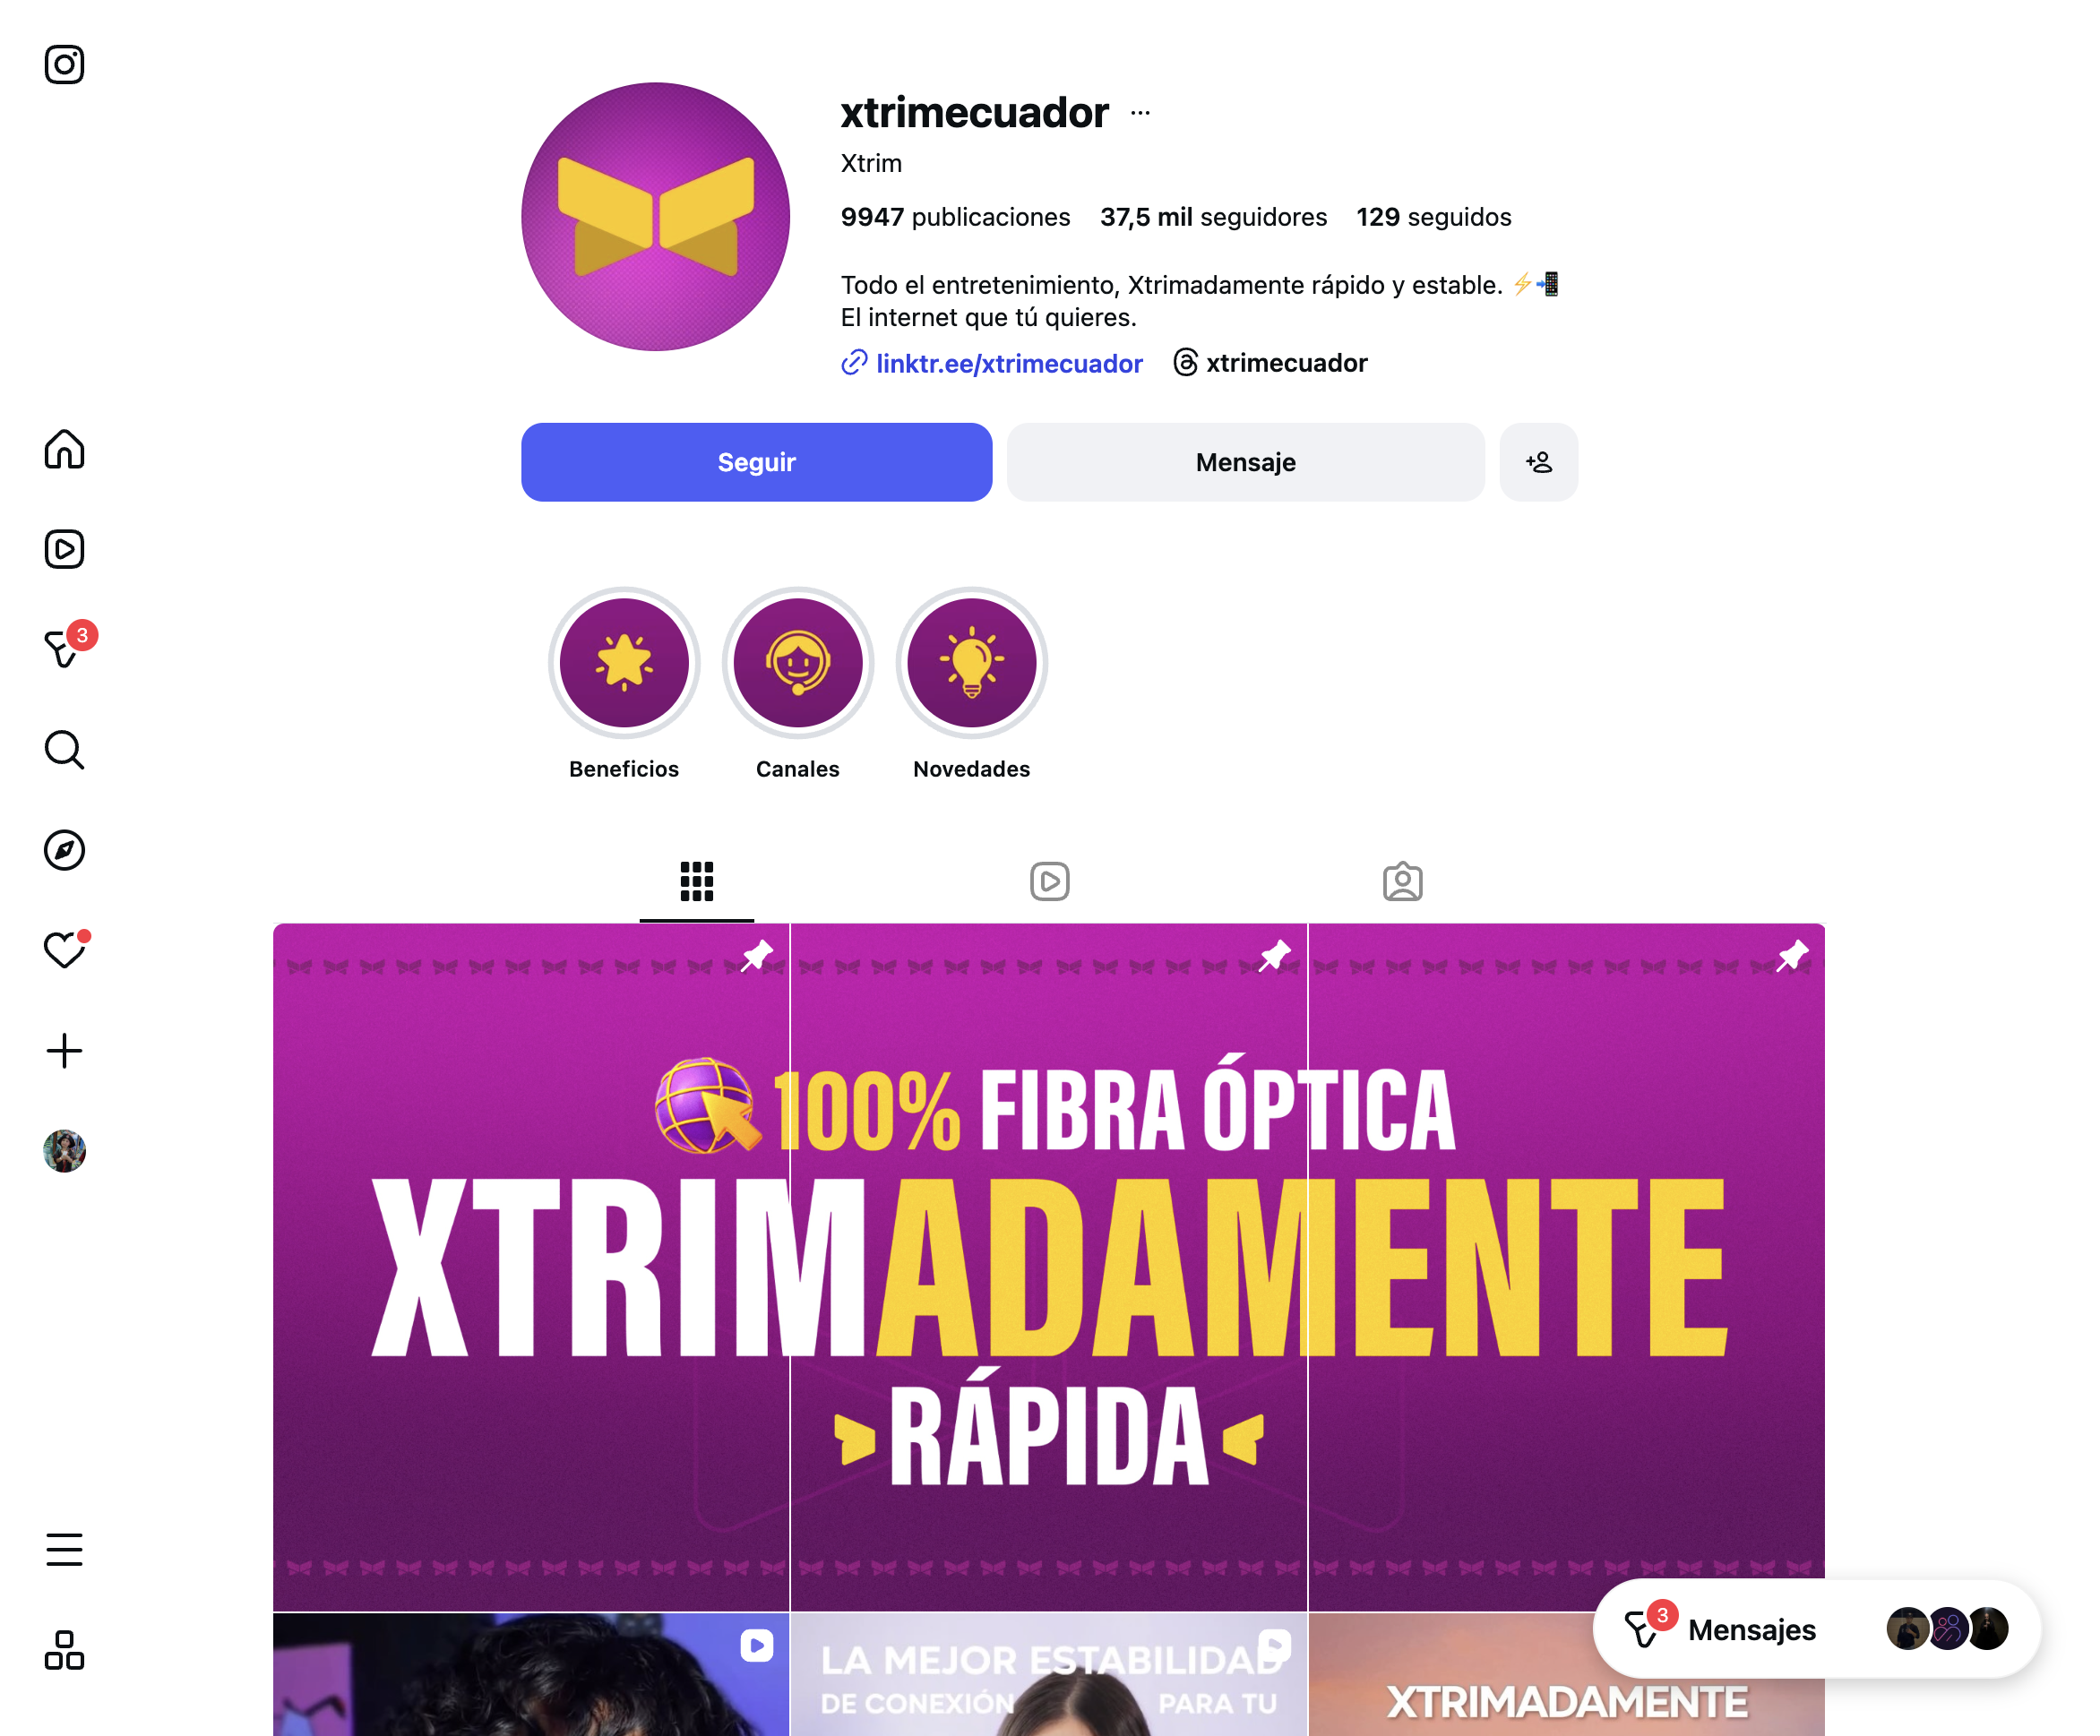
\includegraphics[width=\linewidth]{fig-instagram-xtrim-20260505-v1.png}
  \caption{Instagram de Xtrim Ecuador. Origen: \url{https://www.instagram.com/xtrimecuador/}. Fecha: 2026-05-05.}
\end{figure}

\section{Fuentes y limitaciones}
\subsection{Fuentes usadas (\texttt{observado})}
\begin{itemize}
  \item Sitios oficiales: NETPLUS, Velocity, Celerity, CNT, Vilcanet, Netlife, Xtrim, Snel.
  \item Redes: Facebook de Velocity, Celerity, CNT, Vilcanet, Xtrim; Instagram de Xtrim.
  \item Evidencia visual local: \texttt{docs/reports/figures/netplus-loja/fig-*-20260505-v1.png}
\end{itemize}

\subsection{Limitaciones (\texttt{observado})}
\begin{itemize}
  \item No se confirmo perfil oficial de Facebook para NETPLUS en la URL evaluada.
  \item No se capturo Instagram oficial verificable para todas las marcas en esta corrida.
  \item El componente Google Maps no quedo consolidado en capturas validas dentro de esta ejecucion.
  \item Precios pueden variar por promociones, zona de cobertura y temporalidad comercial.
\end{itemize}

\end{document}
